\chapter{积分}
\section{Riemann积分}
\precis{划分,轴平行矩形及其体积,Riemann积分的定义,Riemann和,Darboux上和,Darboux下和,加细,积分Darboux定理,上积分与下积分,一般有界集上的Riemann积分,Jordan测度,有界集的体积,Jordan可测,Riemann可积的充要条件}
\begin{theorem}{}{C81}
设\(f\)是Jordan可测的有界集\(E\)上的有界函数, 则\(f\)在\(E\)上Riemann可积当且仅当对于任何\(\varepsilon>0\), 存在\(E\)的划分\(P\), 使得\(U(f;P) - L(f;P)<\varepsilon.\)
\end{theorem}
\begin{quiza}
\woe 说明\textbf{Dirichlet函数}\(D(\cdot)=\chi_{\mathbb{Q}}(\cdot)\)在\([0,1]\)上不Riemann可积.
\begin{proof}
	任取划分\(P:0=x_0<x_1<\cdots<x_n=1\), 总能在区间\((x_{i},x_{i+1})\)找到一无理数或有理数, 这意味着\[\lowint_0^1D(x)\dd x=0,\qquad\upint_0^1D(x)\dd x=1,\]从而不Riemann可积.
\end{proof}
\woe 在\(\mathbb{R}\)上定义\textbf{Riemann函数}:\[R(x)=\begin{cases}
          \frac{1}{p},\quad &x=\frac{q}{p},p\in \mathbb{Z}_+,q\in\mathbb{Z}-\{0\},p,q\text{既约},\\
          1,&x=0,\\
          0,&x\notin \mathbb{Q}.
\end{cases}\]证明Riemann函数在\([0,1]\)上Riemann可积.
\begin{proof}
	由Riemann函数的性质, 对任意给定的\(0<\varepsilon<2\), 在\([0,1]\)上使得\(R(x)>\frac{\varepsilon}{2}\)的点至多只有有限个, 不妨设是\(k\)个, 记为\(0=p_1'<p_2'<\cdots<p_k'=1\). 作\([0,1]\)的划分\[0=x_0<x_1<x_2<\cdots<x_{2k-1}=1,\]使得满足\[\begin{split}
		&p_1'\in[x_0,x_1),x_1-x_0<\frac{\varepsilon}{2k},\\
		&p_i'\in(x_{2i-2},x_{2i-1}),x_{2i-1}-x_{2i-2}<\frac{\varepsilon}{2k},i=2,3,\cdots,k-1,\\
		&p_k'\in(x_{2k-2},x_{2k-1}),x_{2k-1}-x_{2k-2}<\frac{\varepsilon}{2k},
	\end{split}\]
设\(\omega_i\)为区间\((x_{i-1},x_i)\)上的振幅, \(\Delta x_i=x_i-x_{i-1}\) 由于\[\sum_{i=1}^{2k-1}\omega_i\Delta x_i=\sum_{j=0}^{k-1}\omega_{2j+1}\Delta x_{2j+1}+\sum_{j=1}^{k-1}\omega_{2j}\Delta x_{2j},\]上式右侧第一个和式中, 有\(\Delta x_{2j+1}<\frac{\varepsilon}{2k}\)且\(\omega_{2j+1}\leqslant 1\), 在第二个和式中, 有\(\omega_{2j}\leqslant\frac{\varepsilon}{2}\)且\(\sum_{j=1}^{k-1}\Delta x_{2j}<1\), 因此得到\(\sum_{i=1}^{n}\omega_i\Delta x_i<k\frac{\varepsilon}{2k}+\frac{\varepsilon}{2}=\varepsilon\). 从而Riemann可积.
\end{proof}
\woe 设\(E\in\mathbb{R}^n\)为Jordan可测的有界闭集, \(f\)为\(E\)上的有界函数, 则\(f\)在\(E\)上Riemann可积当且仅当\(f\)在\(E^{\circ}\)上Riemann可积. 进一步, 当\(f\)在\(E\)上Riemann可积时,\[\int_E f(\boldsymbol{x})\dd\boldsymbol{x}=\int_{E^\circ}f(\boldsymbol{x})\dd x.\]
\begin{proof}
	
\end{proof}
\woe 设\(E\in\mathbb{R}^n\)为Jordan可测的有界闭集, \(f\)为\(E\)上的连续函数. 试用定理\reff{Th:C81}证明\(f\)在\(E\)上Riemann可积.
\begin{proof}
	
\end{proof}
\woe 设\(E\in\mathbb{R}^n\)为Jordan可测的有界闭集, \(f,g\)在\(E\)上Riemann可积, 且\(\int_Ef(\boldsymbol{x})g(\boldsymbol{x})\dd\boldsymbol{x}\ne 0\). 证明: 存在矩形\(R_0\subset E\)使得\(|f|\)在\(R_0\)上有正下界.
\begin{proof}
	
\end{proof}
\woe 设\(E\)是\(\mathbb{R}^n\)中的一个轴平行矩形, 试构造\(E\)上的一个有界恒正函数\(f\), 使得\(\lowint_Ef(\boldsymbol{x})\dd\boldsymbol{x}=0\).
\begin{solution}
	
\end{solution}
\end{quiza}
\begin{quizb}
\woe 设\(f\)是\([a,b]\)上的有界实函数, 对于\([a,b]\)的划分\(P:a=x_0<x_1<x_2<\cdots<x_m=b\), 定义\(W(f;P)=\sum_{k=1}^{m}f(x_k)(x_{k}-x_{k-1})\). 证明: \(f\)在\([a,b]\)上Riemann可积当且仅当\(\lim_{\left\|P\right\|\rightarrow 0^+ }W(f;P)\)存在.
\begin{proof}
	
\end{proof}
\end{quizb}
\section{Lebesgue测度与Lebesgue可测函数}
\precis{Lebesgue外测度,Lebesgue测度,可测集,Carath\'{e}odory条件,几乎处处,\(\sigma\)代数,上限集,下限集,极限集,Borel集,二进方体,不可测集,Lebesgue可测函数,Borel可测函数,简单函数,Carath\'{e}odory函数,依测度收敛,Egorov定理,Riesz定理,Luzin定理}
\begin{theorem}{}{C82}
设\(E\subseteq \mathbb{R}^n\)可测, 则\begin{quizs}
\item 对于任何\(\varepsilon>0\), 存在开集\(G\supseteq E\), 使得\(m(G\backslash E)<\varepsilon\).
\item 对于任何\(\varepsilon>0\), 存在闭集\(F\subseteq E\), 使得\(m(E\backslash F)<\varepsilon\).
\item 存在一列开集\(\{G_k\}\)使得\(G=\bigcap_{k=1}^{\infty}G_k\supseteq E\)且\(G\backslash E\)为零测集.
\item 存在一列闭集\(\{F_k\}\)使得\(F=\bigcup_{k=1}^{\infty}F_k\subseteq E\)且\(E\backslash F\)为零测度集.
\end{quizs}
\end{theorem}
\begin{quiza}
\woe 设\(\mathscr{M}\)为非空集\(X\)上的代数, 即\(\mathscr{M}\)满足以下条件:\begin{compactenum}[(i)]
    \item \(\varnothing,X\in\mathscr{M}\).
    \item 若\(E\in\mathscr{M}\), 则\(X\backslash E\in\mathscr{M}\).
    \item 对任何\(K\geqslant 1\), 若\(E_k\in \mathscr{M}(1\leqslant k\leqslant K)\), 则\(\bigcup_{k=1}^{K}E_k\in\mathscr{M}\).
    \end{compactenum}
证明: \(E_k\in\mathscr{M}(1\leqslant k\leqslant K)\)蕴涵\(E_1\backslash E_2,\bigcap_{k=1}^{K}E_k\in\mathscr{M}\).
\begin{proof}
需要使用De Morgan(德摩根)定律: 设有集合\(X\), 以及集族\(\{A_{\alpha}|\alpha\in I\}\), 则成立\[X\backslash\bigcup_{\alpha\in I}A_{\alpha}=\bigcap_{\alpha\in I}\left(X\backslash A_{\alpha}\right),\qquad X\backslash\bigcap_{\alpha\in I}A_{\alpha}=\bigcup_{\alpha\in I}\left(X\backslash A_{\alpha}\right).\]

由于\(E_1\in\mathscr{M}\), 则\(X\backslash E_1\in\mathscr{M}\), 于是\(\left(X\backslash E_1\right)\cup E_2\in\mathscr{M}\), 注意到\[E_1\backslash E_2=E_1\cap\left(X\backslash E_2\right) X\backslash\left(\left(X\backslash E_1\right)\cup E_2\right)\in\mathscr{M}.\]

诸\(E_k\in\mathscr{M}\), 有\(X\backslash E_k\in \mathscr{M}(1\leqslant k\leqslant K)\), 有\(\bigcup_{k=1}^K\left(X\backslash E_k\right)\in \mathscr{M}\), 于是\(X\backslash\left(\bigcup_{k=1}^K\left(X\backslash E_k\right)\right)\in\mathscr{M}\), 也即\(\bigcap_{k=1}^{K}E_k\in\mathscr{M}\).
\end{proof}
\woe 设\(\mathscr{M}\)为非空集\(X\)上的\(\sigma\)代数. 证明: \(E_k\in\mathscr{M}(k\geqslant 1)\)蕴涵\(\bigcap_{k=1}^{\infty}E_k\in\mathscr{M}.\)
\begin{proof}
	参考上一题.
\end{proof}
\woe 设\(E\subseteq\mathbb{R}^n\). 把定理\reff{Th:C82}的结果一般化为如下结果:
\begin{quizs}
\item 对于任何\(\varepsilon>0\), 存在开集\(G\supseteq E\), 使得\(mG\leqslant m^*E+\varepsilon.\)
\item 对于任何\(\varepsilon>0\), 存在闭集\(F\subseteq E\), 使得\(mF\geqslant m_*E<\varepsilon\).
\item 存在一列开集\(\{G_k\}\)使得\(G=\bigcap_{k=1}^{\infty}G_k\supseteq E\)且\(mG=m^*E\).
\item 存在一列闭集\(\{F_k\}\)使得\(F=\bigcup_{k=1}^{\infty}F_k\subseteq E\)且\(mF=m_*E\).
\end{quizs}
\woe 设\(E\subseteq\mathbb{R}^n\)为Lebesgue可测集, \(f:E\rightarrow [-\infty,+\infty]\)Lebesgue可测. 证明: \(\{f=+\infty\}\)可测.
\begin{proof}
	
\end{proof}
\woe 设\(E\subseteq\mathbb{R}^n\)有界, 则对任何开集\(G\supseteq E\), 有\(m_*E=mG-m^*(G\backslash E)\).
\begin{proof}
	
\end{proof}
\woe 设\(E\subseteq\mathbb{R}^n\), 则\(E\)可测等价于以下任一条件.
\begin{compactenum}[(1)]
\item 对于任何\(\varepsilon>0\), 存在开集\(G\supseteq E\), 使得\(m^*(G\backslash E)<\varepsilon\).
\item 对于任何\(\varepsilon>0\), 存在可测集\(G\supseteq E\), 使得\(m^*(G\backslash E)<\varepsilon\).
\item 对于任何\(\varepsilon>0\), 存在闭集\(F\subseteq E\), 使得\(m^*(E\backslash F)<\varepsilon\).
\item 对于任何\(\varepsilon>0\), 存在可测集\(F\subseteq E\), 使得\(m^*(E\backslash F)<\varepsilon\).
\end{compactenum}
\begin{proof}
	
\end{proof}
\woe 证明: 对于任意\(\varepsilon\in(0,1)\), 存在\([0,1]\)的测度不小于\(1-\varepsilon\)的子集为疏朗集.
\begin{proof}
	
\end{proof}
\woe 证明: 存在\(f\in C[0,1]\), 使得\(\{f=0\}\)为正测度的疏朗集.
\begin{proof}
	
\end{proof}
\woe 设\(E\subseteq\mathbb{R}^n\)可测, \(|E|=+\infty\). 举例说明, 有\(E\)上的可测函数列\(\{f_k\}\)在\(E\)上几乎处处收敛于\(f\), 但\(\{f_k\}\)并非依测度收敛于\(f\).
\begin{proof}
	
\end{proof}
\woe 设\(E\subseteq\mathbb{R}^n\)和\(F\subseteq\mathbb{R}^m\)可测, 证明: \(E\times F\subseteq\mathbb{R}^{n+m}\)可测.
\begin{proof}
	
\end{proof}
\woe 设\(E\subseteq\mathbb{R}^n\)和\(F\subseteq\mathbb{R}^m\)Borel可测, 证明: \(E\times F\subseteq\mathbb{R}^{n+m}\)Borel可测.
\begin{proof}
	
\end{proof}
\woe 证明:\begin{quizs}
\item \(\mathscr{B}(\mathbb{R}^n)\)是由全体以有理点为心, 正有理数为半径的开球生成的\(\sigma\)代数.
\begin{proof}
	
\end{proof}
\item \(\mathscr{B}(\mathbb{R}^n)\)是由\[2^k\left(\left(j_1,j_2,\cdots,j_n\right)^\mathrm{T}+[0,1)^n\right),\quad j_1,j_2,\cdots,j_n,k\in\mathbb{Z},\]定义的全体半开半闭的二进方体\(\mathscr{G}_{DQ}\)生成的\(\sigma\)代数.
\begin{proof}
	
\end{proof}
\end{quizs}
\woe 证明: \(\mathbb{R}^n\)中所有开集组成的集族的势是\(\aleph\).
\begin{proof}
	
\end{proof}
\end{quiza}
\begin{quizb}
\woe 设\(B\)为\(\mathbb{R}^{n+m}\)中的Borel集. 证明对任何\(\boldsymbol{y}\in\mathbb{R}^m\), 截集\(E_{\boldsymbol{y}}=\{\boldsymbol{x}\big|(\boldsymbol{x},\boldsymbol{y})\in B\}\)为\(\mathbb{R}^n\)中得Borel集.
\woe 阅读文献[20], 并按照文献提供的方法证明\(\mathscr{B}(\mathbb{R}^n)\)的势是\(\aleph\).
\woe 考察已经得到的结果中, 相关集合的测度由有限改为无限, 以及函数的取值由实数变为广义实数时, 相应的结果十分仍然成立.
\end{quizb}
 \section{Lebesgue积分及其性质}
\precis{Lebesgue积分,可积函数空间,本性上界,本性下界,绝对可积性,绝对连续性,积分第一中值定理,平行多面体的体积公式,连续型(积分型)H\"{o}lder不等式,权函数,积分型Minkowski不等式,L\'{e}vy单调收敛定理,Fatou引理,Lebesgue控制收敛定理,\(L^p\)空间的完备性}
\begin{quiza}
\woe 对于可测集\(E\)上的函数列\(\{f_k\}\), 说明以下两者等价:\begin{compactenum}[(i)]
\item \(f_k(\boldsymbol{x})\geqslant 0,\mathrm{a.e. }\boldsymbol{x}\in E,\,\forall k\geqslant 1\).
\item \(f_k(\boldsymbol{x})\geqslant 0,\,\forall k\geqslant 1\mathrm{a.e. }\boldsymbol{x}\in E.\).
\end{compactenum}
\woe 设\(f:\mathbb{R}^{n+k}\rightarrow\mathbb{R}\), 说明以下两者不等价:\begin{compactenum}[(i)]
\item \(f(\boldsymbol{x},\boldsymbol{y})\geqslant 0,\mathrm{a.e.\,}\boldsymbol{x}\in\mathbb{R}^n,\,\forall\boldsymbol{y}\in\mathbb{R}^k.\)
\item \(f(\boldsymbol{x},\boldsymbol{y})\geqslant 0,\forall\boldsymbol{y}\in\mathbb{R}^k,\mathrm{a.e.\,}\boldsymbol{x}\in\mathbb{R}^n.\)
\end{compactenum}
\woe 设\(\boldsymbol{f}:\mathbb{R}^n\times\mathbb{R}^{m}\rightarrow\mathbb{R}^k\)可积. 证明: 存在可积的简单函数列\(\{\boldsymbol{f}_j\}\)使得\(\{\boldsymbol{f}_j\}\)逐点收敛于\(\boldsymbol{f}\), 且\(|\boldsymbol{f_k}|\leqslant|\boldsymbol{f}|.\)
\woe 设\(f:\mathbb{R}^n\times\mathbb{R}^m\rightarrow [0,+\infty]\)可测. 证明: 存在可积得简单函数列\(\{f_j\}\)使得\(\{f_j\}\)单调增加, 且逐点收敛于\(f\).
\woe 试用离散型H\"{o}lder不等式证明连续型H\"{o}lder不等式.
\woe 试用连续型H\"{o}lder不等式证明离散型H\"{o}lder不等式.
\woe 证明: \(\lim_{n\rightarrow+\infty}\int_{0}^{\pi}\sin^nx\dd x=0.\)
\begin{proof}
对任给\(0<\varepsilon<1,0<\sin\left(\frac{\pi}{2}-\varepsilon\right)<1\), 故有\[\lim_{n\rightarrow+\infty}\sin^n\left(\frac{\pi}{2}-\varepsilon\right)=0.\]于是存在\(n_0\), 当\(n>n_0\)时, 有\(\sin^n\left(\frac{\pi}{2}-\varepsilon\right)<\varepsilon\). 因而当\(n>n_0\)时,\[\begin{split}
0&\leqslant\int_{0}^{\pi/2}\sin^nx\dd x=\int_{0}^{\pi/2-\varepsilon}\sin^nx\dd x+\int_{\pi/2-\varepsilon}^{\pi/2}\sin^nx\dd x\leqslant\int_{0}^{\pi/2-\varepsilon}\sin^n\left(\frac{\pi}{2}-\varepsilon\right)+\int_{\pi/2-\varepsilon}^{\pi/2}\dd x\\&\leqslant\int_{0}^{\pi/2-\varepsilon}\varepsilon\dd x+\varepsilon\leqslant\left(\frac{\pi}{2}+1\right)\varepsilon,
\end{split}\]所以\(\lim_{n\rightarrow+\infty}\int_{0}^{\pi}\sin^nx\dd x=0.\)
\end{proof}
\woe 设\(E\)为\(\mathbb{R}^n\)上的可测集, \(\boldsymbol{\varphi}:E\rightarrow\mathbb{R}^k\)可测. 证明: \(\{(\boldsymbol{x},\boldsymbol{\varphi}(\boldsymbol{x}))\big|\boldsymbol{x}\in E\}\)是\(\mathbb{R}^{n+k}\)中的零测度集.
\woe 试构造非Jordan可测得有界区域.
\end{quiza}
\begin{quizb}
\woe 在例8.3.2中, 当\(|E|=+\infty\)或(及)\(\left\|f\right\|_{\infty}=+\infty\)时, 结论会如何?
\woe 设\(1\leqslant p<+\infty, E\supseteq\bbr^n\)为测度非零的可测集. 举例说明在\(L^p(E)\)中\begin{quizs}
\item 致密性定理不成立.
\item 聚点原则不成立.
\item 有限覆盖定理不成立.
\end{quizs}
\woe 试构造区间\([0,1]\)上的连续实函数\(f\), 使得\(\{f>0\}\)为可列个两两不交的开区间\(\{\alpha_k,\beta_k\}\)的并, 且若\(f\)在两个不同区间\((\alpha_k,\beta_k)\)和\((\alpha_j,\beta_j)\)上恒为正, \(\beta_k<\alpha_j\), 总存在\(\xi\in(\beta_k,\alpha_j)\)满足\(f(\xi)<0\).
\woe 试构造区间\([a,b]\)上的连续函数\(f\), 以及\([c,d]\)上的Riemann可积函数\(g\), 使得\(g\circ f\)在\([a,b]\)上不Riemann可积, 其中\(f\)的值域包含于\([c,d]\).
\woe 试构造区间\([a,b]\)上的连续函数\(f\), 使得\(g\)在\([a,b]\)上不Riemann可积, 其中\[g(x)=\begin{cases}
f(x),\quad&f(x)\geqslant 1,\\
0,& f(x)<1.
\end{cases}\]
\woe 试构造非Jordan可测的有界闭区域.
\woe 设\(E\subset\bbr^n\)为Jordan可测的有界集, 非负函数\(f\)在\(E\)上Riemann可积, 且\(\int_E f(\boldsymbol{x})\dd\boldsymbol{x}=0.\) 证明: \(\{f\ne 0\}\)是零测度集. 举例说明\(\{f\ne 0\}\)可以不是Jordan可测集.
\end{quizb}
\section{Newton-Lebibiniz公式}
\precis{微积分基本定理---Newton-Lebibiniz公式,定积分的分布积分,定积分的变量代换,带积分余项的Taylor公式,Wallis公式,Stirling公式}
\begin{quiza}
\woe 计算下列积分:\vspace{8pt}\\
\begin{tabular}{lcl}
\((1)\,\int_{0}^{1}x\ee^x\dd x\);&\qquad\qquad\qquad&\((2)\,\int_{0}^{2\pi}\ee^x\sin x\dd x\);\vspace{0.3cm}\\
\((3)\,\int_{0}^{1}\frac{\sqrt{x}+1}{1+x^2}\dd x\);&&\((4)\,\int_{0}^{1}\frac{1}{1+x^3}\dd x\);\vspace{0.3cm}\\
\((5)\,\int_{0}^{\pi}\frac{x}{1+\sin^2x}\dd x\).&&\vspace{0.3cm}\\
\end{tabular}
\tcbline
前两个题较简单, 结果分别1与\(\frac{1}{2}-\frac{\ee^{2\pi}}{2}\), 这里略去过程.
\tcbline

对于\(\int_{0}^{1}\frac{\sqrt{x}+1}{1+x^2}\dd x\), 易见\(\int_{0}^{1}\frac{1}{1+x^2}\dd x=\frac{\pi}{4}\), 我们仅需计算\(\int_{0}^{1}\frac{\sqrt{x}}{1+x^2}\dd x\), 置\(\sqrt{x}=t\), 于是有\(\int_{0}^{1}\frac{\sqrt{x}}{1+x^2}\dd x=\int_{0}^{1}\frac{2t^2}{1+t^4}\dd t\), 因为\[1+t^4=(t^2+1)^2-\left(\sqrt{2}t\right)^2=\left(t^2+\sqrt{2}t+1\right)\left(t^2-\sqrt{2}t+1\right),\]所以\[\frac{2t^2}{1+t^4}=\frac{1}{\sqrt{2}}\cdot\frac{t}{t^2-\sqrt{2}t+1}-\frac{1}{\sqrt{2}}\cdot\frac{x}{x^2+\sqrt{2}x+1},\]从而\[\int\frac{2t^2}{1+t^4}=\frac{1}{2\sqrt{2}}\ln\frac{x^2-\sqrt{2}x+1}{x^2+\sqrt{2}x+1}+\frac{\sqrt{2}}{2}\arctan\left(\sqrt{2}x+1\right)+\frac{\sqrt{2}}{2}\arctan\left(\sqrt{2}x-1\right)+C.\]于是\[\int_{0}^{1}\frac{2t^2}{1+t^4}\dd t=\frac{1}{2\sqrt{2}}\ln\left(3-2\sqrt{2}\right)+\frac{\sqrt{2}}{4}\pi.\]于是\(\int_{0}^{1}\frac{\sqrt{x}+1}{1+x^2}\dd x=\frac{1}{4}\left(\pi+\sqrt{2}\left(\pi+\ln\left(3-2\sqrt{2}\right)\right)\right)\).
\tcbline

对于\(\int_{0}^{1}\frac{1}{1+x^3}\dd x\), 我们有\[\begin{split}
\int_{0}^{1}\frac{1}{1+x^3}\dd x&=\int_{0}^{1}\frac{1}{(1+x)(1-x+x^2)}\dd x=\int_{0}^{1}\left(\frac{1}{3}\cdot\frac{1}{1+x}+\frac{1}{3}\cdot\frac{2-x}{x^2-x+1}\right)\dd x\\&=\left.\frac{1}{3}\ln\left|x+1\right|-\frac{1}{6}\ln(x^2-x+1)+\frac{1}{\sqrt{3}}\arctan\left(\frac{2x-1}{\sqrt{3}}\right)\right|^1_0\\&=\frac{1}{3}\ln 2+\frac{\pi}{3\sqrt{3}}.
\end{split}\]
\tcbline

对于\(\int_{0}^{\pi}\frac{x}{1+\sin^2 x}\dd x\), 易见\[\int_{0}^{\pi}\frac{x}{1+\sin^2x}\dd x=\int_{0}^{\pi}\frac{\pi-x}{1+\sin^2x}\dd x=\frac{\pi}{2}\int_{0}^{\pi}\frac{1}{1+\sin^2x}\dd x,\]对于右侧的积分, 我们有\[\begin{split}
\int_{0}^{\pi}\frac{1}{1+\sin^2x}\dd x&=2\int_{0}^{\pi/2}\frac{1}{1+\sin^2x}\dd x=2\int_{0}^{\pi/2}\frac{\sec^2x}{2\tan^2x+1}\dd x\\&=2\int_{0}^{+\infty}\frac{1}{2t^2+1}\dd t=\frac{\pi}{\sqrt{2}}.
\end{split}\]从而\(\int_{0}^{\pi}\frac{x}{1+\sin^2 x}\dd x=\frac{\pi^2}{2\sqrt{2}}\).
\tcbline
\woe 采用恰当的方法计算下列积分:\vspace{8pt}\\
\begin{tabular}{lcl}
\((1)\,\int_{0}^{1}(1-x)^6x^2\dd x\);&\qquad\qquad\qquad&\((2)\,\int_{0}^{\pi}\sin^4x\cos^2x\dd x\);\vspace{0.3cm}\\
\((3)\,\int_{-1}^{1}x\ee^{x^4}\dd x\);&&\((4)\,\int_{0}^{\pi/2}\frac{\sin x}{\sin x+\cos x}\dd x\);\vspace{0.3cm}\\
\((5)\,\int_{0}^{\pi/2}\frac{\sin x\cos x}{\sin x+\cos x}\dd x\).&&\vspace{0.3cm}\\
\end{tabular}
\begin{solution}
(1)\(\int_{0}^{1}(1-x)^6x^2\dd x=\int_{0}^{1}x^6(1-x)^2\dd x=\int_{0}^{1}\left(x^6-2x^7+x^8\right)\dd x=\frac{1}{252}\).

(2)我们有必要计算\(I_n:=\int_0^\pi \sin^nx\dd x\). 它有如下递推公式\[\begin{split}
\int_0^\pi \sin^nx\dd x&=\int_{0}^{\pi}\sin^{n-1}x\cdot\sin x\dd x=\int_{0}^{\pi}\sin^{n-1}x\dd\left(-\cos x\right)\\&=\int_{0}^{\pi}\left(\sin^{n-1}x\right)'\cos x\dd x=(n-1)\int_{0}^{1}\sin^{n-2}x\left(1-\sin^2x\right)\dd x\\&=(n-1)\int_{0}^{\pi}\sin^{n-2}x\dd x-(n-1)\int_{0}^{1}\sin^nx\dd x\\&=(n-1)I_{n-2}-(n-1)I_n.
\end{split}\]于是\(nI_n=(n-1)I_{n-2}\), 又\(I_2=\int_{0}^{\pi}\sin^2x\dd x=\frac{1}{2}\int_{0}^{\pi}(\sin^2x+\cos^2x)\dd x=\frac{\pi}{2}\), 有\[\int_{0}^{\pi}\sin^4x\cos^2x\dd x=\int_{0}^{\pi}\left(\sin^4x-\sin^6x\right)\dd x=I_4-I_6=\frac{\pi}{16}.\]

(3)易见\(\int_{-1}^{1}x\ee^{x^4}\dd x=0.\)

(4)易见\[\int_{0}^{\pi/2}\frac{\sin x}{\sin x+\cos x}\dd x=\int_{0}^{\pi/2}\frac{\cos x}{\sin x+\cos x}\dd x=\frac{1}{2}\int_{0}^{\pi/2}\frac{\sin x+\cos x}{\sin x+\cos x}\dd x=\frac{\pi}{4}.\]

(5)我们有\(\int_{0}^{\pi/2}\frac{\sin x\cos x}{\sin x+\cos x}\dd x=\int_{0}^{\pi/2}\frac{\left(\sin x+\cos x\right)^2-1}{2(\sin x+\cos x)}\dd x\), 于是\[\begin{split}
&\int_{0}^{\pi/2}\frac{\left(\sin x+\cos x\right)^2-1}{2(\sin x+\cos x)}\dd x=\frac{1}{2}\int_{0}^{\pi/2}(\sin x+\cos x)\dd x-\frac{1}{2}\int_{0}^{\pi/2}\frac{1}{\sin x+\cos x}\dd x\\
=&1-\frac{1}{2}\int_{0}^{\pi/2}\frac{1}{\sqrt{2}}\csc \left(x+\frac{\pi}{4}\right)\dd x=1-\frac{1}{2\sqrt{2}}\int_{\pi/4}^{3\pi/4}\csc x\dd x=1-\frac{1}{2\sqrt{2}}\ln\left(\frac{2+\sqrt{2}}{2-\sqrt{2}}\right).\qedhere
\end{split}\]
\end{solution}
\woe 对于\([a,b]\)上连续可微函数\(f\), 若\(f(a)=f(b)=0\), 证明:\[\max_{a\leqslant x\leqslant b}|f'(x)|\geqslant\frac{4}{(b-a)^2}\left|\int_{a}^{b}f(x)\dd x\right|.\]
\begin{proof}
令\(t=\frac{a+b}{2}+\frac{a-b}{4}\), 于是\[\begin{split}
\left|\int_{a}^{b}f(x)\dd x\right|&=\left|\int_{a}^{b}f(x)\dd (x-t)\right|=\left|f(x)(x-t)\big|^b_a-\int_{a}^{b}f'(x)(x-t)\dd t\right|\\&=\left|\int_{a}^{b}f'(x)\dd t\right|\leqslant \max_{a\leqslant x\leqslant b}|f'(x)|\int_{a}^{b}(x-t)\dd x=\frac{(b-a)^2}{4}\max_{a\leqslant x\leqslant b}|f'(x)|.\qedhere
\end{split}\]
\end{proof}
\woe 证明对任何\(x>0\)成立\(\int_{0}^{x}\ee^{-x^2}\sin x\dd x>0.\)
\begin{proof}
只需证明对于任何自然数\(n\), 有\[\int_{2n\pi}^{(2n+1)\pi}\ee^{-x^2}\sin x\dd x+\int_{(2n+1)\pi}^{(2n+2)\pi}\ee^{-x^2}\sin x\dd x>0,\]注意上述不等式加号左侧的积分大于零而右侧积分小于零. 只有有上述结果, 那么\(\forall x> 0\), 都存在\(k\in\bbn\)使得\(2k\pi\leqslant x\leqslant (2k+1)\pi\)或\((2k+1)\pi\leqslant x\leqslant (2k+2)\pi\), 对于前者, 我们有\[\int_{0}^{x}\ee^{-t^2}\sin t\dd t=\sum_{j=0}^{k-1}\left(\int_{2j\pi}^{\left(2j+1\right)\pi}\ee^{-t^2}\sin t\dd t+\int_{\left(2j+1\right)\pi}^{2\left(j+1\right)\pi}\ee^{-t^2}\sin t\dd t\right)+\int_{2k\pi}^{x}\ee^{-t^2}\sin t\dd t>0,\]对于后者有\[\begin{split}
\int_{0}^{x}\ee^{-t^2}\sin t\dd t=&\sum_{j=0}^{k-1}\left(\int_{2j\pi}^{\left(2j+1\right)\pi}\ee^{-t^2}\sin t\dd t+\int_{\left(2j+1\right)\pi}^{2\left(j+1\right)\pi}\ee^{-t^2}\sin t\dd t\right)\\+&\int_{2k\pi}^{(2k+1)\pi}\ee^{-t^2}\sin t\dd t+\int_{(2k+1)\pi}^{x}\ee^{-t^2}\sin t\dd t>0.
\end{split}\]

事实上,\[\int_{2n\pi}^{(2n+1)\pi}\ee^{-x^2}\sin x\dd x+\int_{(2n+1)\pi}^{(2n+2)\pi}\ee^{-x^2}\sin x\dd x=\int_{2n\pi}^{(2n+1)\pi}\sin t\left(\ee^{-x^2}-\ee^{-(x+\pi)^2}\right)>0.\]结论即证.
\end{proof}
\woe 设\(f\)在\([a,b]\)上有二阶导数, \(f(a)=f(b)=0\). 证明: 存在\(\xi\in(a,b)\)使得\(\int_{a}^{b}f(x)\dd x=\frac{f''(\xi)}{12}(a-b)^3.\)
\begin{proof}
一方面, 我们有
\begin{equation}\tag{$\blacklozenge$}\label{reno1}
\begin{split}
\int_{a}^{b}f(x)\dd x&=\int_{a}^{b}f(x)\dd(x-a)=-\int_{a}^{b}f'(x)(x-a)\dd (x-b)\\&=\int_{a}^{b}f''(x)(x-a)(x-b)\dd x=\frac{f''(\xi_1)}{6}(a-b)^3.
\end{split}
\end{equation}
其中\(\xi_1\in(a,b)\). 另一方面\[\begin{split}
\int_{a}^{(a+b)/2}f(x)\dd x&=\int_{a}^{(a+b)/2}f(x)\dd\left(x-\frac{a+b}{2}\right)=-\int_{a}^{(a+b)/2}f'(x)\left(x-\frac{a+b}{2}\right)\dd (x-a)\\&=\int_{a}^{(a+b)/2}f''(x)\left(x-\frac{a+b}{2}\right)(x-a)\dd x=\frac{f''(\xi_2)}{48}(a-b)^3.
\end{split}\]其中\(\xi_2\in\left(a,\frac{a+b}{2}\right)\), 同理不难得到\[\int_{(a+b)/2}^{b}f(x)\dd x=\frac{f''(\xi_3)}{48}(a-b)^3.\]其中\(\xi_3\in\left(\frac{a+b}{2},b\right)\). 值得一提的是\[\min\{f''(\xi_2),f''(\xi_3)\}\leqslant\frac{f''(\xi_2)+f''(\xi_3)}{2}\leqslant\max\{f''(\xi_2),f''(\xi_3)\},\] 于是依微分Darboux定理有\(f''(\xi_4)=\frac{f''(\xi_2)+f''(\xi_3)}{2}\), 于是有\[\int_{a}^{b}f(x)\dd x=\frac{f''(\xi_4)}{24}(a-b)^3,\] 于是有\(\frac{f''(\xi_1)}{6}=\frac{f''(\xi_4)}{24}\), 易见\(f''(\xi_1),f''(\xi_4)\)同号, 不妨设均非负, 于是有\[f''(\xi_1)\leqslant 2f''(\xi_1)\leqslant  4f''(\xi_1)=f''(\xi_4),\]依微分Darboux定理有\(\xi\)使得\(f(\xi)=2f''(\xi_1)\), 代入即式\eqref{reno1}即得结论.
\end{proof}
\woe 设\(f\)是\([0,1]\)上的连续函数. 证明\(f(0)=0\)时, \(f(y)=\int_{0}^{1}\frac{y^3f(x)}{x^4+y^4}\dd x\)在\(y=0\)处连续.
\begin{proof}
若\(f(0)=0\), 则记\[M=\max_{x\in[0,1]}\left|f(x)\right|,\quad\omega(r)=\sup_{0\leqslant x\leqslant r}\left|f(x)\right|,\quad r\geqslant 0.\]
\(\forall y\ne 0\), 我们有\[\begin{split}
\left|F(y)-F(0)\right|=&\left|F(y)\right|=\left|\int_{0}^{1}\frac{y^3f(x)}{x^4+y^4}\dd x\right|\leqslant\int_{0}^{1}\frac{|y^3||f(x)|}{x^4+y^4}\dd x\\\leqslant&\omega(r)\int_{0}^{r}\frac{|y^3|}{x^4+y^4}\dd x+M\int_{r}^{1}\frac{|y^3|}{x^4+y^4}\dd x\\=&\omega(r)\int_{0}^{r/|y|}\frac{1}{1+x^4}\dd x+M\int_{r/|y|}^{1/|y|}\frac{1}{1+x^4}\dd x,
\end{split}\]上式令\(y\rightarrow 0\)得到\[\varlimsup_{y\rightarrow 0}|F(y)-F(0)|\leqslant\omega(r)\int_{0}^{+\infty}\frac{\dd x}{1+x^4},\quad\forall r\in (0,1),\]令\(r\rightarrow 0^+\), 则有\[\varlimsup_{y\rightarrow 0}|F(y)-F(0)|\leqslant 0,\]即\(\lim_{y\rightarrow 0}F(y)=F(0).\)

事实上, 在上述我们证明了\[\lim_{y\rightarrow 0}\left|\int_{0}^{1}\frac{y^3f(x)}{x^4+y^4}\dd x-\int_{0}^{1}\frac{y^3f(0)}{x^4+y^4}\dd x\right|=0,\]即\[\lim_{y\rightarrow 0^+}\int_{0}^{1}\frac{y^3f(x)}{x^4+y^4}\dd x=\lim_{y\rightarrow 0^+}\int_{0}^{1}\frac{y^3f(0)}{x^4+y^4}\dd x=\lim_{y\rightarrow 0^+}\int_{0}^{1/y}\frac{f(0)}{1+x^4}\dd x=\int_{0}^{+\infty}\frac{f(0)}{1+x^4}\dd x,\]这样就有\(\lim_{y\rightarrow 0^-}\int_{0}^{1}\frac{y^3f(x)}{x^4+y^4}\dd x=\int_{0}^{+\infty}\frac{f(0)}{1+x^4}\dd x=\frac{\pi}{2\sqrt{2}}f(0).\) 由\(F(0)=0\), 我们得到\(F\)在0处连续当且仅当\(f(0)=0\).
\end{proof}
\woe 已知\(f\in C^1[0,+\infty)\), 且存在\(c>0\)使得\(|f'(x)|\leqslant\frac{c}{x}(\forall x>0),\lim_{R\rightarrow+\infty}\frac{1}{R}\int_{0}^{R}|f(x)|\dd x=0\). 证明: \(\lim_{x\rightarrow+\infty}f(x)=0\).
\begin{proof}
由题设易见\(\lim_{x\rightarrow+\infty}f'(x)=0\), 于是对于\(\forall A>0\), 对于充分大的\(x\), 有\[f(x+A)-f(x)=f'(\xi)A,\quad \xi\in(x,x+A),\]于是\(\lim_{x\rightarrow+\infty}|f(x)|\)存在, 记为\(a\). 于是对\(\forall\varepsilon>0\), 存在\(R'\)使得\(x\geqslant R'\)使得\[\left||f(x)|-a\right|<\varepsilon,\quad\text{即}\quad a-\varepsilon\leqslant |f(x)|\leqslant a+\varepsilon,\]
由于\(\frac{1}{R}\int_{0}^{R}|f(x)|\dd x=\frac{1}{R}\int_{0}^{R'}|f(x)|\dd x+\frac{1}{R}\int_{R'}^{R}|f(x)|\dd x\), 于是
\[\frac{1}{R}\int_{0}^{R'}|f(x)|\dd x+\frac{1}{R}\int_{R'}^{R}(a-\varepsilon)\dd x\leqslant\frac{1}{R}\int_{0}^{R}|f(x)|\dd x\leqslant\frac{1}{R}\int_{0}^{R'}|f(x)|\dd x+\frac{1}{R}\int_{R'}^{R}(a+\varepsilon)\dd x,\]令\(R\rightarrow+\infty\)得到\(\lim_{R\rightarrow+\infty}\frac{1}{R}\int_{0}^{R}|f(x)|\dd x=a\), 结合题设得\(a=0\).
\end{proof}
\woe 设\(E\subseteq\bbr^n\). 证明: \(f:E\rightarrow[-\infty,+\infty]\)为下半连续函数当且仅当对任何\(\alpha\in\bbr,\{f>\alpha\}\)是\(E\)中的相对开集.
\woe 设\(E\subseteq\bbr^n\).\begin{quizs}
\item 若\(\varphi,\psi:E\rightarrow(-\infty,+\infty]\)均为下半连续函数, 证明: \(\varphi+\psi\)也是下半连续函数.
\item 若\(\varphi,\psi:E\rightarrow[-\infty,+\infty)\)均为上半连续函数, 证明: \(\varphi+\psi\)也是上半连续函数.
\end{quizs}
\woe 设\(E\subseteq\bbr^n\).\begin{quizs}
\item 若\(\varphi_k:E\rightarrow[-\infty,+\infty](k\geqslant 1)\)为一列下半连续函数, 证明: \(\varphi=\sup_{k\geqslant 1}\varphi_k\)也是下半连续函数.
\item 若\(\varphi_k:E\rightarrow[-\infty,+\infty](k\geqslant 1)\)为一列上半连续函数, 证明: \(\varphi=\inf_{k\geqslant 1}\varphi_k\)也是上半连续函数.
\end{quizs}
\woe 设\(E\subseteq\bbr^n\). 证明: \(f:E\rightarrow\bbr\)连续当且仅当它既是下半连续的, 又是上半连续的.
\woe 证明: 紧集上有下界的下半连续函数有最小值.
\end{quiza}
\begin{quizb}
\woe 试构造区间\([a,b]\)上处处可导且导函数有界的实函数\(f\), 使得\(f'\)在\([a,b]\)上不是Riemann可积的.
\begin{solution}
    
\end{solution}
\woe 试构造\([0,1]\)上的可积函数\(f\), 使得对任何有理数\(q\in[0,1]\), 都有\(\lim_{x\rightarrow q}f(x)=+\infty\).
\begin{solution}
    
\end{solution}
\woe 试构造\(\bbr\)上严格单调的连续可微函数\(f\), 使得\(\{f'=0\}\)具有正测度.
\woe 设\(n\geqslant 1, f\in C[0,1]\)且满足\(\int_{0}^{1}x^kf(x)\dd x=0,k=0,1,\cdots,n-1,\int_{0}^{1}f(x)x^n\dd x=1.\) 证明: \(\max_{x\in[0,1]}|f(x)|>2^n(n+1)\).
\begin{proof}
由题意知对任意\(\alpha\in\bbr\), 有\[\int_{0}^{1}\left(x-\alpha\right)^nf(x)\dd x=1,\]若对于\(f(x)\)恒有\(|f(x)|<2^n(n+1)\), 则\[\begin{split}
\int_{0}^{1}\left(x-\frac{1}{2}\right)^nf(x)\dd x\leqslant\int_{0}^{1}\left|x-\frac{1}{2}\right|^n|f(x)|\dd x<2^n(n+1)\int_{0}^{1}\left|x-\frac{1}{2}\right|^n=1,
\end{split}\]与题设矛盾, 即必有使得\(|f(x)|\geqslant 2^n(n+1)\)的点, 即\(\max_{x\in[0,1]}|f(x)|\geqslant 2^n(n+1)\). 若\(\max_{x\in[0,1]}f(x)=2^n(n+1)\), 则依上式取等的条件必有\(|f(x)|\equiv 2^n(n+1)\), 这与题设矛盾.
\end{proof}
\woe 设\(f\in C[0,\pi]\), 且对\(1\leqslant k\leqslant n\)成立\(\int_{0}^{\pi}f(x)\cos kx\dd x=\int_{0}^{\pi}f(x)\sin kx\dd x=0\). 证明: \(f\)在\((0,\pi)\)内至少有\(2n\)个零点.
\woe 设\(f\in C[a,b]\)非负, 且在\(c\in[a,b]\)处取得唯一的最大值\(f(c)>0,\varphi\)在\([a,b]\)上可积, 且在点\(c\)连续, 证明: \[\lim_{n\rightarrow+\infty}\frac{\displaystyle\int_{a}^{b}f^n(x)\varphi(x)\dd x}{\displaystyle\int_{a}^{b}f^n(x)\dd x}=\varphi(c).\]
\begin{proof}
由于\(\varphi\)在\(c\)点连续, 则\(\forall \varepsilon>0\)使得\(|x-c|<\delta\)时, \(|\varphi(x)-\varphi(c)|<\varepsilon\), 并且\(\delta\)也满足\(|x-c|\geqslant\delta\)时有\(0\leqslant f(x)<f(c)-\varepsilon\). 即\(f(c)\)与\(|\varphi|\)的最大值为\(M\)与\(m\). 又存在\(\eta\)使得\(|x-c|\leqslant\eta\)时, \(|f(x)-f(c)|<\frac{\varepsilon}{2}\), 记\(E\)为区间\([a,b]\)去除\([c-\delta,c+\delta]\)的部分. 于是有\[\begin{split}
&\left|\frac{\displaystyle\int_{a}^{b}f^n(x)\varphi(x)\dd x}{\displaystyle\int_{a}^{b}f^n(x)\dd x}\right|\leqslant\frac{\displaystyle\int_{a}^{b}f^n(x)|\varphi(x)-\varphi(c)|\dd x}{\displaystyle\int_{a}^{b}f^n(x)\dd x}\\\leqslant&\frac{\displaystyle\int_{c-\delta}^{c+\delta}f^n(x)|\varphi(x)-\varphi(c)|\dd x}{\displaystyle\int_{c-\delta}^{c+\delta}f^n(x)\dd x}+\frac{\displaystyle\int_{E}f^n(x)|\varphi(x)-\varphi(c)|\dd x}{\displaystyle\int_{c-\eta}^{c+\eta}f^n(x)\dd x}\\\leqslant&\frac{\varepsilon\displaystyle\int_{c-\delta}^{c+\delta}f^n(x)\dd x}{\displaystyle\int_{c-\delta}^{c+\delta}f^n(x)\dd x}+\frac{2(b-a-2\delta)m(M-\varepsilon)^n}{2\eta(M-\varepsilon/2)^2}\rightarrow \varepsilon,\quad n\rightarrow 0.
\end{split}\]
令\(\varepsilon\rightarrow 0^+\), 原命题得证.
\end{proof}
\woe 计算\(\lim_{n\rightarrow+\infty}\frac{n\displaystyle\int_{0}^{\pi/2}x^n\cos x\dd x}{\displaystyle\int_{0}^{\pi/2}x^n\sin x\dd x}.\)
\begin{solution}
注意到\[\int_{0}^{\pi/2}x^n\sin x\dd x=-x^n\cos x\big|_0^{\pi/2}+n\int_{0}^{\pi/2}x^{n-1}\cos x\dd x,\]即有\(\lim_{n\rightarrow+\infty}\frac{n\displaystyle\int_{0}^{\pi/2}x^n\cos x\dd x}{\displaystyle\int_{0}^{\pi/2}x^n\sin x\dd x}=\lim_{n\rightarrow+\infty}\frac{\displaystyle\int_{0}^{\pi/2}x^n\cos x\dd x}{\displaystyle\int_{0}^{\pi/2}x^{n-1}\cos x\dd x}=\frac{\pi}{2}.\)
\end{solution}
我们来证明这样一个命题: 设\(f,\varphi\in C[a,b]\), 且\(f,\varphi>0\), 则\[\lim_{n\rightarrow+\infty}\frac{\displaystyle\int_{a}^{b}\varphi(x)f^{n+1}(x)\dd x}{\displaystyle\int_{a}^{b}\varphi(x)f^n(x)\dd x}=\max_{x\in[a,b]}f(x).\]
\begin{proof}
记\(M=\max_{x\in[a,b]}f(x)=f(x_0)\), 则\(\forall\varepsilon\in\left(0,\frac{M}{2}\right),\exists\delta>0\), 使得当\(x\in J_\varepsilon:=(x_0-\delta,x_0+\delta)\cap[a,b]\)时, 有\(f(x)>M-\varepsilon\). 令\[g(x)=\max\{f(x,M-2\varepsilon)\},\quad x\in[a,b].\]则\(g\)连续且\[|g^k(x)-f^k(x)|\leqslant (M-2\varepsilon)^k,\quad\forall x\in[a,b],k=1,2,\cdots.\]
于是我们有\[\varlimsup_{n\rightarrow+\infty}\frac{\left|\displaystyle\int_{a}^{b}\varphi(x)\left(f^{n+1}(x)-g^{n+1}(x)\right)\dd x\right|}{\displaystyle\int_{a}^{b}\varphi(x)f^n(x)\dd x}\leqslant\varlimsup_{n\rightarrow+\infty}\frac{(M-2\varepsilon)^{n+1}\displaystyle\int_{a}^{b}\varphi(x)\dd x}{(M-\varepsilon)^n\displaystyle\int_{J_{\varepsilon}}\varphi(x)\dd x}=0.\]
从而可得\[\varliminf_{n\rightarrow+\infty}\frac{\displaystyle\int_{a}^{b}\varphi(x)f^{n+1}(x)\dd x}{\displaystyle\int_{a}^{b}\varphi(x)f^n(x)\dd x}=\varliminf_{n\rightarrow+\infty}\frac{\displaystyle\int_{a}^{b}\varphi(x)g^{n+1}(x)\dd x}{\displaystyle\int_{a}^{b}\varphi(x)f^n(x)\dd x}\geqslant M-2\varepsilon.\]
这样, 由\(\varepsilon\)的任意性得到\(\varliminf_{n\rightarrow+\infty}\frac{\displaystyle\int_{a}^{b}\varphi(x)f^{n+1}(x)\dd x}{\displaystyle\int_{a}^{b}\varphi(x)f^n(x)\dd x}\geqslant M\), 另一方面\[\varlimsup_{n\rightarrow+\infty}\frac{\displaystyle\int_{a}^{b}\varphi(x)f^{n+1}(x)\dd x}{\displaystyle\int_{a}^{b}\varphi(x)f^n(x)\dd x}\leqslant M,\]从而上述命题成立.
\end{proof}
\woe 求极限: \(\lim_{n\rightarrow+\infty}\frac{\displaystyle\int_{0}^{1}\left(1-\frac{x}{2}\right)^n\left(1-\frac{x}{4}\right)^n\dd x}{\displaystyle\int_{0}^{1}\left(1-\frac{x}{2}\right)^n\dd x}\).
\begin{solution}
注意到\[\int_{0}^{1}\left(1-\frac{x}{2}\right)^n\dd x=\frac{2}{n+1}\left(1-\frac{1}{2^{n+1}}\right)\sim\frac{2}{n+1},\quad n\rightarrow+\infty,\]
对于\(\int_{0}^{1}\left(1-\frac{x}{2}\right)^n\left(1-\frac{x}{4}\right)^n\dd x\), 置\(t=nx\)得\[\int_{0}^{1}\left(1-\frac{x}{2}\right)^n\left(1-\frac{x}{4}\right)^n\dd x=n\int_{0}^{n}\left(1-\frac{t}{2n}\right)^n\left(1-\frac{1}{4n}\right)^n\dd t,\]
于是由Lebesgue控制收敛定理有\[\begin{split}
\lim_{n\rightarrow+\infty}\frac{\displaystyle\int_{0}^{1}\left(1-\frac{x}{2}\right)^n\left(1-\frac{x}{4}\right)^n\dd x}{\displaystyle\int_{0}^{1}\left(1-\frac{x}{2}\right)^n\dd x}=&\lim_{n\rightarrow+\infty}\frac{1}{2}\int_{0}^{+\infty}\left(1-\frac{t}{2n}\right)^n\left(1-\frac{1}{4n}\right)^n\chi_{[0,n]}(t)\dd t\\=&\frac{1}{2}\int_{0}^{+\infty}\ee^{-3t/4}\dd t=\frac{2}{3}.\qedhere
\end{split}\]
\end{solution}
\woe 试将一些微分中值定理型的问题转化成积分中值定理型的结果, 并考察其异同.
\end{quizb}
设\(f(x)\)在区间\([0,1]\)有连续的导函数, 且\(f(0)=0\), 求证:\[\int_{0}^{1}|f(x)|^2\dd x\leqslant\frac{1}{2}\int_{0}^{1}(1-x^2)|f'(x)|^2\dd x,\]等号成立当且仅当\(f(x)=\equiv cx\), 其中\(c\)为常数.
\begin{proof}
由\(f(0)=0\)可知\(f(x)=\int_{0}^{x}f'(t)\dd t,x\in[0,1]\), 由Cauchy不等式可得\[f^2(x)=\left(\int_{0}^{x}f'(t)\dd t\right)^2\leqslant \int_{0}^{x}\left(f'(t)\right)^2\dd t\cdot\int_{0}^{x}1^2\dd t=x\int_{0}^{x}\left(f'(t)\right)^2\dd t,\]
于是有\[\begin{split}
\int_{0}^{1}f^2(x)\dd x&\leqslant\int_{0}^{1}\left(x\int_{0}^{x}\left(f'(t)\right)^2\dd t\right)\dd x=\int_{0}^{1}\left(\int_{0}^{x}\left(f'(t)\right)^2\dd t\right)\dd\left(-\frac{1-x^2}{2}\right)\\
&=-\frac{1-x^2}{2}\int_{0}^{x}\left(f'(t)\right)^2\dd t\Big|_0^1+\int_{0}^{1}\frac{1-x^2}{2}\left(f'(x)\right)^2\dd x\\&=\frac{1}{2}\int_{0}^{1}(1-x^2)\left(f'(x)\right)^2\dd x.
\end{split}\]
其中等号成立当且仅当\(\left(\int_{0}^{x}f'(t)\dd t\right)^2\leqslant \int_{0}^{x}\left(f'(t)\right)^2\dd t\cdot\int_{0}^{x}1^2\dd t\)恒成立, 故此时有\(f'(t)=c\), 结合\(f(0)=0\)即得\(f(x)=cx\).
\end{proof}
\section{累次积分}
\precis{累次积分,Fubuni定理,积分型Young不等式及其推广}
\begin{theorem}{Young不等式}{young}
设\(\varphi\)是\(\left[,+\infty\right]\)上的严格单增的连续函数, \(\varphi(0)=0,\varphi(+\infty)=+\infty,\psi\)是\(\varphi\)的反函数, 令\[\varPhi(x)=\int_0^x\varphi(t)\dd t,\qquad\varPsi(y)=\int_{0}^{y}\psi(t)\dd t,\quad x,y\geqslant 0,\]则对任何\(a,b\geqslant 0\)成立\[ab\leqslant\varPhi(a)+\varPsi(b),\]且等号当且仅当\(b=\varphi(a)\), 即\(a=\psi(b)\)时取到.
\end{theorem}
\begin{quiza}
\woe 计算积分\(\iiint_\varOmega \frac{\dd x\dd y \dd z}{(1+x+y+z)^3}\), 其中\(\varOmega\)为平面\(x=0,y=0,z=0\)和\(x+y+z=1\)所围成的有界区域.
\begin{solution}
将重积分化为累次积分, 即有\[\begin{split}
&\iiint_{\varOmega}\frac{\dd x\dd y\dd z}{(1+x+y+z)^3}=\int_{0}^{1}\dd x\int_{0}^{1-x}\dd y\int_{0}^{1-x-y}\frac{1}{(1+x+y+z)^3}\dd z\\=&\int_{0}^{1}\dd x\int_{0}^{1-x}\left(\frac{1}{2(1+x+y)^2}-\frac{1}{8}\right)\dd y=\int_{0}^{1}\left(\frac{1}{2(1+x)}-\frac{1-x}{8}-\frac{1}{4}\right)\dd x\\=&\frac{1}{2}\ln 2-\frac{5}{16}.\qedhere
\end{split}\]
\end{solution}
\woe 计算积分\(\iiint_\varOmega z^2\dd x\dd y \dd z\), 其中\(\varOmega\)为\(x^2+y^2+z^2\leqslant 1\)与\(x^2+y^2+z^2\leqslant 2z\)相交的部分.
\begin{solution}
注意到被积函数仅含\(z\), 于是有\[\iiint_{\varOmega}z^2\dd x\dd y\dd z=\int_{0}^{1/2}\pi z^2\left(2z-z^2\right)\dd z+\int_{1/2}^{1}\pi z^2\left(1-z^2\right)=\frac{29\pi}{480}.\qedhere\]
\end{solution}
\woe 设\(R>0\), 计算牟合方盖\(\{(x,y,z)\big|x^2+y^2\leqslant R^2,y^2+z^2\leqslant R^2\}\)的体积.
\begin{solution}
记\(D=\{(x,y,z)\big|x^2+y^2\leqslant R^2,y^2+z^2\leqslant R^2\}\), 考虑到对称性, 我们只计算图形第一象限部分的体积. 注意到该区域边界当\(y\)确定时, 总有\(x^2=z^2=R^2-y^2\), 记\(D_{xz}\)为\(y\)确定后代表的区域, 于是\[\begin{split}
\iiint_{D}\dd x\dd y\dd z=\int_{0}^{R}\left(\iint_{D_{xz}}\dd x\dd z\right)\dd y=\int_{0}^{R}\left(R^2-y^2\right)\dd y=\frac{2}{3}R^3.
\end{split}\]从而牟合方盖的体积\(V=8\cdot\frac{2}{3}R^3=\frac{16}{3}R^3.\)
\end{solution}
\woe 当\(\varphi\)连续可导时, 利用求导得到单调性来证明定理\reff{Th:young}.
\begin{proof}

\end{proof}
\woe 设\(f,g\)在\([0,1]\)上单调. 若\(f,g\)均单增或均单减, 证明: \(\int_0^1f(x)g(x)\dd x\geqslant\int_{0}^{1}f(x)\dd x\int_{0}^{1}g(x)\dd x\). 若\(f,g\)之一单增, 另一个单减, 则上述不等式的不等号反向.
\begin{proof}
若\[\int_{0}^{1}f(x)g(x)\dd x\geqslant\int_{0}^{1}f(x)\dd x\int_{0}^{1}g(x)\dd x,\]则有\[\int_{0}^{1}\int_{0}^{1}f(x)g(x)\dd x\dd y=\int_{0}^{1}\int_{0}^{1}f(x)g(y)\dd x\dd y\]即有\[\int_{0}^{1}\int_{0}^{1}\left(f(x)g(x)-f(x)g(y)\right)\dd x\dd y=\int_{0}^{1}\int_{0}^{1}\left(f(y)g(y)-f(y)g(x)\right)\dd x\dd y\geqslant 0.\]即证\[\int_{0}^{1}\int_{0}^{1}\left(f(x)g(x)+f(y)g(y)-f(x)g(y)-f(y)g(x)\dd x\dd y\right)\geqslant 0.\]结合\(f,g\)的单调性与排序不等式可知上式成立, 另外的情况同理可以得到.
\end{proof}
\woe 求证\(\int_{0}^{1}\sqrt[3]{\frac{\ln(1+x)}{x}}\dd x\int_{0}^{1}\sqrt[3]{\frac{\ln^2(1+x)}{x^2}}\dd x<\frac{\pi^2}{12}\).
\begin{proof}
利用基本不等式, 有\[\begin{split}
\int_{0}^{1}\sqrt[3]{\frac{\ln (1+x)}{x}}\dd x\int_{0}^{1}\sqrt[3]{\frac{\ln^2(1+x)}{x^2}}\dd x&=\int_{0}^{1}\int_{0}^{1}\sqrt[3]{\frac{\ln (1+x)}{x}}\int_{0}^{1}\sqrt[3]{\frac{\ln^2(1+y)}{y^2}}\dd x\dd y\\&<\frac{1}{3}\int_{0}^{1}\int_{0}^{1}\frac{\ln(1+x)}{x}+\frac{\ln(1+y)}{y}+\frac{\ln(1+y)}{y}\dd x\dd y\\&=\int_{0}^{1}\frac{\ln(1+x)}{x}=\frac{\pi^2}{12}.\qedhere
\end{split}\]
\end{proof}
\woe 令\(\varSigma\)为平面直角坐标系中以点\(A(1,0),\,B(0,1),\,C(-1,0),\,D(0,-1)\)为顶点的正方形区域. 证明: \(\left(\iint_\varSigma\ee^{|x|+|y|}\dd x\dd y\right)^{1/2}<2\int_{0}^{\sqrt{2}/2}\ee^x\dd x\).
\begin{proof}
记\(\varSigma_1\)为\(\varSigma\)与第一象限的交, 则由对称性有\[\iint_\varSigma\ee^{|x|+|y|}\dd x\dd y=4\iint_{\varSigma_1}\ee^{x+y}\dd x\dd y.\]记\(\varSigma_2=\left\lbrace(x,y)\big|0\leqslant x,y\leqslant\sqrt{2}/2\right\rbrace\)注意到\[2\int_{0}^{\sqrt{2}/2}\ee^x\dd x=\int_{0}^{\sqrt{2}/2}\ee^x\dd x+\int_{0}^{\sqrt{2}/2}\ee^y\dd y\geqslant 2\sqrt{\iint_{\varSigma_2}\ee^{x+y}\dd x\dd y}\geqslant 2\sqrt{\iint_{\varSigma_1}\ee^{x+y}\dd x\dd y},\]从而结论成立. 最右侧不等号成立的原因为\(\varSigma_2\)与\(\varSigma_1\)面积相同, 但\(x+y\)在\(\varSigma_2\)中的值不小于在\(\varSigma_1\)中的值.
\end{proof}
\woe 设函数\(f\in C[a,b]\), 且\(0<m\leqslant f(x)\leqslant M(\forall x\in[a,b])\). 证明:\[(b-a)^2\leqslant\int_{a}^{b}f(x)\dd x\cdot\int_{a}^{b}\frac{1}{f(x)}\dd x\leqslant\frac{(m+M)^2}{4Mm}(b-a)^2.\]
\begin{proof}
左侧由Cauchy不等式有\[\int_{a}^{b}f(x)\dd x\cdot\int_{a}^{b}\frac{1}{f(x)}\dd x\geqslant\left(\int_{a}^{b}\sqrt{f(x)}\cdot\sqrt{\frac{1}{f(x)}}\dd x\right)^2=(b-a)^2.\]注意到\[0\geqslant\frac{\left(f(x)-M\right)\left(f(x)-m\right)}{f(x)}=f(x)+\frac{Mm}{f(x)}-(M+m),\]即有\[\int_{a}^{b}f(x)\dd x+\int_{a}^{b}\frac{Mm}{f(x)}\dd x\leqslant (M+m)(b-a),\]又\[\int_{a}^{b}f(x)\dd x+\int_{a}^{b}\frac{Mm}{f(x)}\dd x\geqslant 2\sqrt{Mn}\sqrt{\int_{a}^{b}f(x)\dd x\cdot\int_{a}^{b}\frac{1}{f(x)}\dd x},\]从而结论成立.
\end{proof}
\woe 对以下闭区域\(W\), 计算\(E=\{(x,y)\big|\exists x\in\mathbb{R},\,\mathrm{s.t.}\,(x,y,z)\in W\}\), 以及\(F_{y,z}=\{x\big|(x,y,z)\in W\}(\forall(y,z)\in E)\). 进而化\(\iiint_Wf(x,y,z)\dd x\dd y\dd z\)为先对\(x\)积分再对\((y,z)\)积分的累次积分:\begin{compactenum}[(1)]
    \item \(W=\{(x,y,z)\big|x,y\geqslant 0,x+y\leqslant 1,0\leqslant z\leqslant xy\}\);
    \item \(W=\{(x,y,z)\big|x,y\geqslant 0,0\leqslant z\leqslant x+y\leqslant 1\}\).
    \end{compactenum}
\begin{solution}
(1)

(2)
\end{solution}
\end{quiza}
\begin{quizb}
\woe 设\(f\in C(\mathbb{R})\)是双射, 有不动点, 又满足\(f(2x-f(x))=x(\forall x\in\mathbb{R})\). 证明\(f(x)\equiv x\).
\begin{proof}
由题设有\[f(x)+f^{-1}(x)=2x,\quad \forall x\in\bbr.\]设\(g(x)=f(x)-x\), 首先, 归纳证明\[f\left(x+kg(x)\right)=x+\left(k+1\right)g(x),\quad k\in\bbz.\]根据定义, 对\(k=0\)成立. 假设\[f\left(x\pm (k-1)g(x)\right)=x+\pm kg(x),\quad k\in\bbz,\]那么\[\begin{split}
&f(x\pm kg(x))=2\left(x\pm kg(x)\right)-f^{-1}\left(x+\pm kg(x)\right)\\
=&2\left(x\pm kg(x)\right)-x\left(x\pm (k-1)g(x)\right)=x\pm \left(k+1\right)g(x),
\end{split}\]归纳完成.

假设\(g(x)<g(y)\)对于某些\(x,y\in\bbr\)成立, 那么可以选择\(k\in\bbn\)使得\(x-kg(x)>y-kg(y)\). 注意\(f\)是增函数, 否则\(f\)与\(f^{-1}\)是减函数, 这与\(2x=f(x)+f^{-1}(x)\)矛盾. 因此, \(f\)的\(n\)次迭代\(f^{(n)}\)也是一个增函数. 由此可见\[f^{(n)}\left(x-kg(x)\right)\geqslant f^{(n)}\left(y-kg(y)\right),\]由于\(f^{(n)}(x)\left(x-kg(x)\right)=f^{(n-1)}\left(x+(1-k)kg(x)\right)=\cdots=x+(n-k)g(x),\)类似的\[f^{(n)}\left(x-kg(x)\right)=y+(n-k)g(y),\]得到\[x+(n-k)g(x)\geqslant y+(n-k)g(y),\]但这并不适用于所有\(n\)足够大的情况, 否则\[\frac{x}{n-k}+g(x)\geqslant\frac{y}{n-k}+g(y),\]令\(n\rightarrow+\infty\), 得到\(g(x)\geqslant g(y)\)矛盾. 所以\(g(x)\)是常数, 因此\(f(x)=x+c,c\in\bbr\), 又因\(f(x)\)有不动点, 从而\(f(x)\equiv x\). 
\end{proof}
\woe 如果\(\varphi\)是\(\left[0,+\infty\right)\)上单调增加的非负函数, 特别的, \(\varphi(0)\)不一定为零, \(\varphi\)不一定严格单调, 且\(\varphi(+\infty)\)不一定为\(+\infty\). 尝试建立相应的Young不等式.
\begin{proof}

\end{proof}
\woe 设\(f\in C^1[0,h],\,f(0)=f(h)=0\), 证明: \(\int_{0}^{h}\left|f(x)f'(x)\right|\dd x\leqslant\frac{h}{4}\int_{0}^{h}\left|f'(x)\right|^2\dd x\), 且系数\(\frac{h}{4}\)不可改进.
\begin{proof}
由\(f(0)=0\)有\[\left|f(x)\right|=\left|\int_{a}^{x}f'(t)\dd t\right|\leqslant\int_{0}^{x}\left|f'(t)\right|\dd t=:F(x),\]同理由\(f(h)=0\)得到\(\left|f(x)\right|=\left|\int_{h}^{x}f'(t)\dd t\right|\leqslant\int_{h}^{x}\left|f'(t)\right|\dd t=:G(x)\). 于是有\[\begin{split}
\int_{0}^{h}\left|f(x)f'(x)\right|\dd x&=\int_{0}^{h/2}\left|f(x)f'(x)\right|\dd x+\int_{h/2}^{h}\left|f(x)f'(x)\right|\dd x\\&\leqslant\int_{0}^{h/2}F(x)F'(x)\dd x+\int_{h/2}^{h}G(x)G'(x)\dd x\\&=\frac{1}{2}F^2\left(\frac{h}{2}\right)+\frac{1}{2}G^2\left(\frac{h}{2}\right),
\end{split}\]而\[F^2\left(\frac{h}{2}\right)=\left(\int_{0}^{h/2}\left|f'(t)\right|\dd t\right)^2,\quad G^2\left(\frac{h}{2}\right)=\left(\int_{h/2}^{h}\left|f'(t)\right|\dd t\right)^2,\]再由Cauchy-Schwarz不等式\[\left(\int_{0}^{h/2}\left|f'(t)\right|\dd t\right)^2\leqslant\int_{0}^{h/2}1^2\dd x\int_{0}^{h/2}\left|f'(x)\right|^2\dd x=\frac{h}{2}\int_{0}^{h/2}\left|f'(x)\right|^2\dd x,\]同理\(\left(\int_{h/2}^{h}\left|f'(x)\right|\dd t\right)^2\leqslant\frac{h}{2}\int_{h/2}^{h}\left|f'(x)\right|^2\dd x\), 即证原不等式.

等号成立当且仅当\[f(x)=\begin{cases}
cx,\quad& 0\leqslant x\leqslant h/2,\\
-c(x-h),\quad& h/2\leqslant x\leqslant h,
\end{cases}\]上述函数满足\(f(0)=f(h)=0\), 若还要求\(f(x)\)导数连续, 只有取\(f(x)\equiv 0\), 若不然, \(f(x)\)在\(x=\frac{h}{2}\)处不可微, 即知\(\frac{h}{4}\)不能再小. 实际上, 这正是华罗庚-Opial不等式.
\end{proof}
\woe 设\(F\)在\([0,1]\times [0,1]\)上有连续的四阶偏导数, 满足\(\left|\frac{\partial^4F(x,y)}{\partial x^2\partial y^2}\right|\leqslant M,\,F(x,0)=F(x,1)=0=F(0,y)=F(1,y)=0(\forall x,y\in[0,1])\). 证明: \(\left|\int_{[0,1]\times [0,1]}F(x,y)\dd x\dd y\right|\leqslant\frac{M}{144}\).
\begin{proof}
先记\(D=\{(x,y)\big|0\leqslant x,y\leqslant 1\}\), 考虑积分\(\iint_{D}x(1-x)y(1-y)\frac{\partial^4F}{\partial x^2\partial y^2}\dd x\dd y\), 一方面, 有\[\left|\iint_{D}x(1-x)y(1-y)\frac{\partial^4F}{\partial x^2\partial y^2}\dd x\dd y\right|\leqslant\left|M\int_{0}^{1}x(1-x)\dd x\int_{0}^{1}y(1-y)\dd y\right|=\frac{M}{36}.\]另一方面,\[\begin{split}
&\iint_{D}x(1-x)y(1-y)\frac{\partial^4F}{\partial x^2\partial y^2}\dd x\dd y=\int_{0}^{1}\dd x\int_{0}^{1}x(1-x)y(1-y)\frac{\partial^4F}{\partial x^2\partial y^2}\dd y\\=&\int_{0}^{1}\dd x\int_{0}^{1}x(1-x)y(1-y)\dd\left(\frac{\partial^3F}{\partial x^2\partial y}\right)=\int_{0}^{1}\dd x\int_{0}^{1}x(1-x)(2y-1)\frac{\partial^3F}{\partial x^2\partial y}\dd y\\=&\int_{0}^{1}\dd x\int_{0}^{1}x(1-x)(2y-1)\dd\left(\frac{\partial^2F}{\partial x^2}\right)=\int_{0}^{1}\dd x\int_{0}^{1}2x(1-x)\frac{\partial^2F}{\partial x^2}\dd y\\=&2\int_{0}^{1}\dd y\int_{0}^{1}x(1-x)\frac{\partial^2F}{\partial x^2}\dd x=4\int_{0}^{1}\dd x\int_{0}^{1}F(x,y)\dd y=4\iint_{D}F(x,y)\dd x\dd y,
\end{split}\]从而有\(4\left|\int_{[0,1]\times [0,1]}F(x,y)\dd x\dd y\right|\leqslant\frac{M}{36}\). 即得结论.
\end{proof}
\end{quizb}
\section{重积分变量代换}
\precis{重积分变量代换,Jacobi矩阵(行列式),(广义)极坐标变换,(广义)柱面坐标变换,旋转体的体积,(广义)球面坐标变换,(广义)高维球面坐标变换}
\begin{quiza}
\woe 计算\(\iiint\limits_{4x^2+4y^2+z^2\leqslant 4x+4y+z}\left(4x^2+4y^2+z^2\right)\dd x\dd y\dd z\).
\begin{solution}
记原积分为\(I\), 于是
\begin{align}
I&=\iiint\limits_{4(x-1/2)^2+4(y-1/2)^2+(z-1/2)^2\leqslant 9/4}\left(4x^2+4y^2+z^2\right)\dd x\dd y\dd z\tag{整理}\\
&=\iiint\limits_{4x^2+4y^2+z^2\leqslant 9/4}\left(4\left(x+\frac{1}{2}\right)^2+4\left(y+\frac{1}{2}\right)^2+\left(z+\frac{1}{2}\right)^2\right)\dd x\dd y\dd z\tag{平移变换}\\
&=\iiint\limits_{4x^2+4y^2+z^2\leqslant 9/4}\left(4x^2+4y^2+z^2+\frac{9}{4}\right)\dd x\dd y\dd z\tag{奇数次项积分为0}\\
&=\frac{27}{32}\cdot\frac{9}{4}\iiint\limits_{x^2+y^2+z^2\leqslant 1}\left(x^2+y^2+z^2+1\right)\dd x\dd y\dd z\tag{伸缩变换}
\end{align}
最后利用球坐标变换有\[I=\frac{27}{32}\cdot\frac{9}{4}\int_{0}^{2\pi}\dd\theta\int_{0}^{\pi}\dd\varphi\int_{0}^{1}\left(r^2+1\right)r^2\sin\varphi\dd r=\frac{81\pi}{20}.\qedhere\]
\end{solution}
\woe 计算由\((a_1x+b_1y+c_1)^2+(a_2x+b_2y+c_2)^2=1\)所围成的有界区域\(D\)的面积(其中\(a_1b_2-a_2b_1\ne 0\)).
\begin{solution}
即计算\(\iint_{D}\dd x\dd y\), 令\(u=a_1x+b_1y+c_1,v=a_2x+b_2y+c_2\), 则\[\left|\det\left(\frac{\partial(x,y)}{\partial(u,v)}\right)\right|=\left|\frac{1}{\det\left(\displaystyle\frac{\partial(u,v)}{\partial(x,y)}\right)}\right|=\left|\frac{1}{a_1b_2-a_2b_1}\right|,\]于是\(\iint_{D}\dd x\dd y=\iint_{u^2+v^2\leqslant 1}\frac{1}{|a_1b_2-a_2b_1|}\dd u\dd v=\frac{\pi}{|a_1b_2-a_2b_1|}\).
\end{solution}
\woe 计算积分\(\int_{0}^{1}\dd x\int_{0}^{1-x}\ee^{y/(x+y)}\dd y.\)
\begin{solution}
置\(x+y=u,y=v\), 不难得到\[\int_{0}^{1}\dd x\int_{0}^{1-x}\ee^{y/(x+y)}\dd y=\int_{0}^{1}\dd u\int_{0}^{u}\ee^{v/u}\dd v=\int_{0}^{1}(\ee-1)u\dd u=\frac{1}{2}(\ee-1).\qedhere\]
\end{solution}
\woe 设\(f\)在点0处可导,\(f(0)=0,\varOmega_t=\{(x,y,z)\big|x^2+y^2+z^2\leqslant 2tz\}\).求\(\lim_{t\rightarrow 0^+}\frac{1}{t^5}\iiint_{\varOmega_t}f(x^2+y^2+z^2)\dd x\dd y\dd z\).
\begin{solution}
记原极限为\(I\). 做变量代换\[\begin{cases}
x=r\cos\theta\sin\varphi,\\
y=r\sin\theta\sin\varphi,\\
z=t+r\cos\varphi,
\end{cases}\quad\theta\in[0,2\pi],\varphi\in[0,\pi],r\geqslant 0.\]则当\(t>0\)时,\[\begin{split}
\frac{1}{t^5}\iiint_{\varOmega_t}f(x^2+y^2+z^2)\dd x\dd y\dd z&=\frac{1}{t^5}\int_{0}^{2\pi}\dd\theta\int_{0}^{\pi}\dd\varphi\int_{0}^{t}f(r^2+t^2+2tr\cos\varphi)r^2\sin\varphi\dd r\\
&=\frac{2\pi}{t^2}\int_{0}^{\pi}\dd\varphi\int_{0}^{1}f(t^2r^2+t^2+2t^2r\cos\varphi)r^2\sin\varphi\dd r,
\end{split}\]
对于任何\(t\in(0,1]\), 我们有\[\begin{split}
&\frac{2\pi}{t^2}\int_{0}^{\pi}\dd\varphi\int_{0}^{1}\left|f(t^2r^2+t^2+2t^2r\cos\varphi)-f'(0)(t^2r^2+t^2+2t^2r\cos\varphi)\right|r^2\sin\varphi\dd r\\
\leqslant&\frac{2\pi}{t^2}\int_{0}^{\pi}\dd\varphi\int_{0}^{1}(t^2r^2+t^2+2t^2r\cos\varphi)\omega(t^2r^2+t^2+2t^2r\cos\varphi)r^2\sin\varphi\dd r\\
\leqslant&2\pi\int_{0}^{\pi}\dd\varphi\int_{0}^{1}4\omega\left(4t^2\right)\dd r=8\pi^2\omega\left(4t^2\right),
\end{split}\]
其中\(\omega(r)=\sup_{0<|x|\leqslant r}\left|\frac{f(x)}{x}-f'(0)\right|\)满足\(\lim_{r\rightarrow0^+}\omega(r)=0.\) 所以\[I=\lim_{t\rightarrow 0^+}\frac{2\pi}{t^2}\int_{0}^{\pi}\dd\varphi\int_{0}^{1}f'(0)\left(t^2r^2+t^2+2t^2r\cos\varphi\right)r^2\sin\varphi\dd r=\frac{32\pi}{15}f'(0).\qedhere\]
\end{solution}
\woe 设\(R>0\), 证明: \(\sqrt{\frac{\pi}{4}(1-\ee^{-R^2})}\leqslant\int_{0}^{R}\ee^{-x^2}\dd x\leqslant\sqrt{\frac{\pi}{4}\left(1-\ee^{-4R^2/\pi}\right)}\).
\begin{proof}
记\(P=\{(x,y)\big|x^2+y^2\leqslant R^2,x,y\geqslant 0\},Q=\{(x,y)\big|0\leqslant x,y\leqslant R\}\), 易见\(P\subset Q\), 并且\[\iint_{P}\ee^{-(x^2+y^2)}\dd x\dd y=\int_{0}^{\pi/4}\dd\theta\int_{0}^{R}\ee^{-r^2}r\dd r=\frac{\pi}{4}\left(1-\ee^{-R^2}\right),\]故\(\frac{\pi}{4}\left(1-\ee^{-R^2}\right)\leqslant\iint_{Q}\ee^{-(x^2+y^2)}\dd x\dd y=\left(\int_{0}^{R}\ee^{-x^2}\dd x\right)^2\). 

\begin{minipage}{0.3\linewidth}
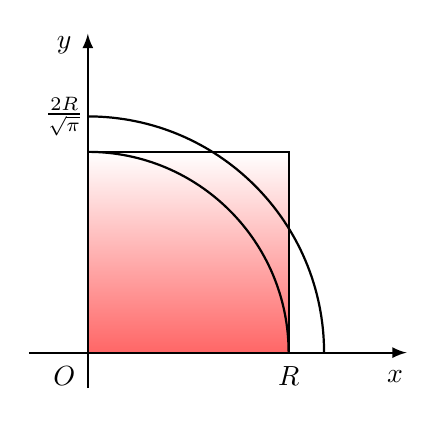
\begin{tikzpicture}[scale=1.5]
\tikzstyle{gray_block} = [draw,outer sep=7,inner sep=7,minimum size=57,line width=1,thick, draw=black, top color=white,bottom color=red!60]
\draw[thick,-latex](-0.5,0)--(2.7,0);
\draw[thick,-latex](0,-0.3)--(0,2.7);
\node at (-0.2,-0.2) {$O$};
\node at (2.6,-0.2) {$x$};
\node at (-0.2,2.6) {$y$};
\draw[thick,gray_block](1.7,0)--(1.7,1.7)--(0,1.7)--(0,0)--(1.7,0);
\draw[thick] (1.7,0) arc (0:90:1.7);
\draw[thick] (2,0) arc (0:90:2);
\node at (1.7,-0.2) {$R$};
\node at (-0.2,2) {$\frac{2R}{\sqrt{\pi}}$};
\end{tikzpicture}
\end{minipage}
\begin{minipage}{0.65\linewidth}
记\(C=\left\lbrace(x,y)\big|x^2+y^2\leqslant 4R^2/\pi,x,y\geqslant 0\right\rbrace\), 易见\(C\backslash Q\)与\(Q\backslash C\)面积相等, 但\[\ee^{-(x^2+y^2)}\geqslant \ee^{-4R^2/\pi},\quad (x,y)\in C\backslash Q,\]
\end{minipage}

而\((x,y)\in Q\backslash C\)时上述不等式反向, 故有\[\begin{split}
\left(\int_{0}^{R}\ee^{-x^2}\dd x\right)^2=\iint_{Q}\ee^{-(x^2+y^2)}\dd x\dd y\leqslant \iint_{C}\ee^{-(x^2+y^2)}\dd x\dd y&=\int_{0}^{\pi/4}\dd\theta\int_{0}^{2R/\sqrt{\pi}}\ee^{-r^2}r\dd r\\
&=\frac{\pi}{4}\left(1-\ee^{4R^2/\pi}\right),
\end{split}\]
从而原不等式成立.
\end{proof}
\end{quiza}
\begin{quizb}
\woe 试求半径为\(R\)密度为常值\(\rho\)的球体对于质量为\(m\)的质点\(P\)的万有引力.
\begin{solution}
首先, 两质量分别为\(m_1,m_2\), 相距为\(r\)的质点之间的引力为\[\boldsymbol{F}=\frac{Gm_1m_2}{r^2},\]其中\(G\)为引力常数, 约为\(6.67\times 10^{-11}N\cdot m^2/kg^2\).

现在, 我们不妨记题设球体为\(D=\{(x,y,z)\big| x^2+y^2+z^2\leqslant R^2\}\), 质点\(P\)坐标为\((0,0,p)\).
\begin{figure}[H]
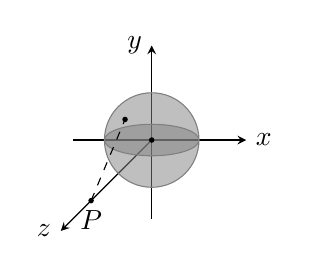
\begin{tikzpicture}[>=stealth]
  \draw [->] (-1,0,0) -- (1.2,0,0) node [at end, right] {$x$};
  \draw [->] (0,-1,0) -- (0,1.2,0) node [at end, left]  {$y$};
  \draw [->] (0,0,0) -- (0,0,3) node [at end, left]  {$z$};
  \begin{scope}[xshift=-0cm,yshift=0cm,,fill opacity=0.5]
\draw[fill, color=gray]  (0,0,0) circle (0.6);
\draw [fill, color=gray] (0,0) ellipse [x radius=0.6cm, y radius=0.2cm];
\end{scope}
\fill (0,0,0) circle (1pt);
\fill (-0.3,0.3,0.1) circle (1pt);
\fill (0,0,2) circle (1pt);
\node at(0,-0.25,2){$P$};
\draw[dashed](0,0,2)--(-0.3,0.3,0.1);
\end{tikzpicture}
\end{figure}
在球中任取一点\(Q(x,y,z)\), 环绕\(Q\)取一体积微元\(\dd V\), \(\dd V\)与\(P\)之间的引力\(\dd\boldsymbol{F}\)为\[\dd \boldsymbol{F}(x,y,z)=\frac{Gm\rho\dd V}{x^2+y^2+(z-p)^2},\]方向由\(P\)指向\(Q\), 我们记\(\angle QPO=\alpha\), 则\(\boldsymbol{F}\)沿\(z\)轴方向与垂直\(z\)轴方向的分量为\[\boldsymbol{F}_1=\boldsymbol{F}\cos\alpha,\quad \boldsymbol{F}_2=\boldsymbol{F}\sin\alpha,\]注意到\(\cos\alpha=\frac{p-z}{\sqrt{x^2+y^2+(z-p)^2}}\), 于是\[\boldsymbol{F}=\iiint_{D}\frac{Gm\rho(p-z)}{(x^2+y^2+(z-l)^2)^{3/2}}\dd V,\]
\end{solution}
\woe 设\(\varOmega\subseteq\mathbb{R}^n\)为区域, \(\psi:\varOmega\rightarrow\mathbb{R}^m\)连续可微. 若\(E\)为\(\varOmega\)的紧子集, 证明: 存在连续模\(\omega\)使得\[\left\|\psi(\boldsymbol{y})-\psi(\boldsymbol{x})-\psi_{\boldsymbol{x}}(\boldsymbol{x})(\boldsymbol{y}-\boldsymbol{x})\right\|\leqslant\left\|\boldsymbol{y}-\boldsymbol{x}\right\|\omega\left(\left\|\boldsymbol{y}-\boldsymbol{x}\right\|\right)\]
\end{quizb}
\section{函数的光滑逼近}
\precis{函数的光滑逼近,支集,简单函数逼近可积函数,连续函数逼近可积函数,\(C^k\)函数一致逼近连续函数,一致收敛,内闭一致收敛,卷积,Young不等式,磨光算子,Weierstrass逼近定理,连续函数的延拓}
\begin{quiza}
\woe 证明函数\[\varphi(x)=\begin{cases}
\ee^{-1/x},\quad &x>0,\\
0,&x\leqslant 0
\end{cases}\]任意次可导.
\begin{proof}
易见\(x\ne 0\)时\(\varphi\)任意次可导. \(x=0\)时有\[\lim_{x\rightarrow 0^+}\frac{\ee^{-1/x}}{x}=0=\lim_{x\rightarrow 0^-}\frac{0-0}{x},\]则\[\varphi'(x)=\begin{cases}
\frac{\ee^{-1/x}}{x^2},\quad,&x>0\\
0&x\leqslant 0.
\end{cases}\]归纳可证\[\varphi^{(n)}(x)=\begin{cases}
P_n\left(\frac{1}{x}\right)\ee^{-1/x},\qquad &x>0,\\
0,&x\leqslant 0.
\end{cases}\]其中\(P_n(x)\)为一\(2n\)次多项式. \(n=1\)已经满足, 设\(\varphi^{(n)}(x)\)如上式所示, 那么\[\lim_{x\rightarrow 0^+}=\frac{\ee^{-1/x}}{x}P_n\left(\frac{1}{x}\right)=\lim_{t\rightarrow+\infty}\frac{tP(t)}{\ee^t}=0,\]且有\[\left(P_n\left(\frac{1}{x}\right)\ee^{-1/x}\right)'=P'_n\left(\frac{1}{x}\right)\ee^{-1/x}+\frac{1}{x^2}P_n(x)\ee^{-1/x}=P_{n+1}(x)\ee^{-1/x},\]从而\(\varphi(x)\)任意次可导.
\end{proof}
\woe 设\(b>a,n>\frac{4}{b-a}\). 证明: 存在\(g_n\in C_c^{\infty}\left((a,b);[0,1]\right)\)满足\(\supp g_n=\left[a+\frac{1}{n},b-\frac{1}{n}\right]\), \(g_n\big|_{\left[a+2/n,b-2/n\right]}\equiv 1\)以及\(|g'|\leqslant nM\), 其中\(M\)是一个与\(n\)无关的一个常数.
\begin{proof}

\end{proof}
\woe 设\(\alpha>0,f\in L_{loc}^1\left(\bbr\right).\) 定义\(F(x)=\frac{1}{\alpha}\int_{x}^{x+\alpha}f(t)\dd t(\forall x\in\bbr)\). 证明:\begin{quizs}
\item 若\(f\)是单调函数, 则\(F\)也是单调函数.
\item 若\(f\)是凸函数, 则\(F\)也是凸函数.
\item 若\(f\)有连续的\(n\)阶导数, 且\(f^{(n)}\geqslant 0\), 则\(F^{(n)}\geqslant 0\).
\end{quizs}
\begin{proof}
	(1)不妨设有连续单增的函数\(g(x)\), 记\(G(x)=\frac{1}{\alpha}\int_{x}^{x+\alpha}g(t)\dd t\), 于是有\[G'(x)=\frac{1}{\alpha}\left(g(x+\alpha)-g(\alpha)\right)\geqslant 0,\]从而对于连续函数, 上述结论成立. 而一般的\(f\in L_{loc}^1\left(\bbr\right)\), 我们知道对于\(\forall\varepsilon>0\), 存在\(g(x)\in C_c(\bbr)\)使得\[\int_{\bbr}|g(x)-f(x)|\dd x\leqslant\varepsilon,\]从而\(\forall x_1>x_2\), 有\[\begin{split}
		&\frac{1}{\alpha}\left|\int_{x_1}^{x_1+\alpha}f(t)\dd t-\int_{x_2}^{x_2+\alpha}f(t)\dd t-\left(\int_{x_1}^{x_1+\alpha}g(t)\dd x-\int_{x_2}^{x_2+\alpha}g(t)\dd t\right)\right|\\
		=&\frac{1}{\alpha}\left|\int_{x_1}^{x_1+\alpha}\left(f(t)-g(t)\right)\dd t-\int_{x_2}^{x_2+\alpha}\left(f(t)-g(t)\right)\dd t\right|\\
		\leqslant&\frac{1}{\alpha}\left(\int_{x_1}^{x_1+\alpha}|g(t)-f(t)|\dd t+\int_{x_2}^{x_2+\alpha}|g(t)-f(t)|\dd t\right)\leqslant\frac{2}{\alpha}\varepsilon.
	\end{split}\]
	有\(\varepsilon\)的任意性可知原命题成立.
\end{proof}
\woe 设\(f\in L_{loc}^{1}\left(\bbr\right),\varphi\in C_{c}^{\infty}\left(\bbr\right)\)非负且恒不为零. 定义\(F=f*\varphi\). 证明对于这样定义的函数\(F\), 也具有第3题中所列的性质.
\woe 若对任何\(x,y\in\bbr\), \(\bbr\)上的一元实函数\(f\)满足\(f(x+y)=f(x)+f(y)\). 进一步, \(f\)在一个区间内有界. 证明: 存在常数\(c\)使得\(f(x)=cx(\forall x\in\bbr)\).
\end{quiza}
\begin{quizb}
\woe 试利用Weierstrass第一逼近定理证明Weierstrass第二逼近定理.
\begin{proof}

\end{proof}
\woe 试利用Weierstrass第二逼近定理证明Weierstrass第一逼近定理.
\begin{proof}

\end{proof}
\woe 将习题\(8.7.\boldsymbol{\mathcal{A}}\)中的第2题推广到高维情形: 设\(D\subset\bbr^n\)为有界区域. 对于\(\delta>0\), 取区域\(\varOmega\)使得\(D\subset\subset \varOmega,\inf_{\boldsymbol{x}\in D,\boldsymbol{y}\in\partial\varOmega}|\boldsymbol{x}-\boldsymbol{y}|\geqslant\delta\). 证明: 存在\(\varphi\in C_c^{\infty}(\varOmega)\), 满足\(0\leqslant\varphi\leqslant 1,\varphi\big|_D\equiv 1\)以及\(|\nabla\varphi|\leqslant\frac{M}{\delta}\), 其中\(M\)是与\(\delta\)无关的一个常数.
\woe 设\(\bbr\)上可测实函数\(f\)满足\(f(x+y)=f(x)+f(y)\). 证明: 存在常数\(c\)使得\(f(x)=cx(\forall x\in\bbr)\).

\textbf{提示: }存在闭集\(E\subset [0,1]\), 使得\(|E|>\frac{3}{4}\)且\(f\)限制在\(E\)上连续. 证明: \(\left(-\frac{1}{2},\frac{1}{2}\right)\subset E-E\).
\woe 设\(\bbr\)上可测实函数\(f\)中点凸. 证明: \(f\)是凸函数.
\woe 在Weierstrass逼近定理的证明中, 一个重要的思想是利用\textbf{Bernstein(伯恩斯坦)多项式}, 设\(f\)是\([0,1]\)上的函数, 其Bernstein多项式定义为\[B_n(f;x)=\sum_{k=0}^{n}C_n^kf\left(\frac{k}{n}\right)x^k(1-x)^{n-k},\quad x\in[0,1].\]试证明:\begin{quizs}
\item 对任何\(x\in[0,1]\), 有\(\sum_{k=0}^{n}C_n^k(k-nx)^2x^k(1-x)^{n-k}=nx(1-x).\)
\item 设\(f\in C[0,1]\), 证明: \(\{B_n(f;x)\}\)在\([0,1]\)上一致收敛到\(f(x)\).
\end{quizs}
\woe 设\(T: C[a,b]\rightarrow C[a,b]\)是线性算子, 若对任何非负的\(f\in[a,b]\), 都有\(Tf\)非负, 则称\(T\)是\textbf{正线性算子}. 试证明如下的\textbf{Korovkin(科罗夫金)定理}: 设\(\{T_n\}\)是\(C[a,b]\rightarrow C[a,b]\)的一列正线性算子, 若对于\(f(x)=1,x,x^2,\{T_nf\}\)均在\([a,b]\)上一致收敛于\(f\), 则对任何\(f\in C[a,b]\), \(\{T_nf\}\)在\([a,b]\)上一致收敛于\(f\).
\woe 验证第5题给出的\(B_n\)是\(C[0,1]\)到\(C[0,1]\)的正线性算子, 且对于\(f(x)=1,x,x^2,\{T_nf\}\)均在\([0,1]\)上一致收敛于\(f\).
\end{quizb}
\section{光滑逼近的应用}
\precis{分部积分公式的推广,带积分型余项Taylor公式的推广,积分第二中值定理,推广的Riemann-Lebesgue引理,无理数之均匀分布}
\begin{theorem}{}{c88}
设\(q,r\)为对偶数, 函数\(g\)以\(T>0\)为周期, \(g\big|_{[0,T]}\in L^r[0,T], f\in L^q[a,b]\), 则\[\lim_{p\rightarrow+\infty}\int_{a}^{b}f(x)g(px)\dd x=\frac{1}{T}\int_{0}^{T}g(x)\dd x\int_{a}^{b}f(x)\dd x.\]
\end{theorem}
\begin{theorem}{}{wuli}
设\(f\)在\([0,1]\)上Riemma可积, \(s\)是无理数, 则\[\lim_{n\rightarrow+\infty}\frac{1}{n}\sum_{k=1}^{n}f\left(\{ks\}\right)=\int_{0}^{1}f(x)\dd x.\]
\end{theorem}
\begin{quiza}
\woe 计算极限\(\lim_{n\rightarrow +\infty}\int_{0}^{1}\frac{x^2|\sin nx|}{1+x^2}\dd x.\)
\begin{solution}
由定理\reff{Th:c88}, 立即可得\[\lim_{n\rightarrow +\infty}\int_{0}^{1}\frac{x^2|\sin nx|}{1+x^2}\dd x=\frac{1}{2\pi}\int_{0}^{2\pi}|\sin x|\dd x\int_{0}^{1}\frac{x^2}{1+x^2}\dd x=\frac{2}{\pi}-\frac{1}{2}.\qedhere\]
\end{solution}
\woe 设\([0,+\infty)\)上的非负连续函数\(f\)单调递减, \(F(x)=\int_{0}^{x}(x-2t)f(t)\dd t(\forall x\geqslant 0)\), 证明\(F\)是\([0,+\infty)\)上的凸函数.
\begin{proof}
我们只需证明\(F'(x)=\int_{0}^{x}f(t)\dd t-xf(x)\)单增, 任取\(0<x_1<x_2\), 则\(f(x_1)\geqslant f(x_2)\), 又\[\begin{split}
F(x_2)-F(x_1)&=\int_{0}^{x_2}f(t)\dd t-x_2f(x_2)-\int_{0}^{x_1}f(x_1)\dd t+x_1f(x_1)\\&=\int_{x_1}^{x_2}f(t)\dd t+x_1f(x_1)-x_2f(x_2)\\&\geqslant (x_2-x_1)f(x_2)+x_1f(x_1)-x_2f(x_2)=x_1\left(f(x_1)-f(x_2)\right)\geqslant 0.
\end{split}\]从而\(F\)为凸函数.
\end{proof}
\woe 设\(g\)为\([a,b]\)上的单调函数, 证明存在\([a,b]\)上连续可导的单调函数列\(\{g_n\}\)使得\(g_n(a)=g(a),g_n(b)=g(b),\max_{x\in [a,b]}|g_n(x)|\leqslant M_g=\max_{x\in [a,b]}|g(x)|\)以及\(\lim_{n\rightarrow+\infty}\int_{a}^{b}|g_n(x)-g(x)|\dd x=0.\)
\begin{proof}

\end{proof}
\woe 将定理\reff{Th:c88} 推广到高维情形. 设\(p,q\)为对偶数, \(E\in\bbr^n\)为有界可测集, \(f\in L^p(E)\). \(Q\)为矩形\([0,a_1]\times [0,a_2]\times\cdots\times [0,a_n]\), 函数\(g\)以\(Q\)为周期, 即对任何\(\boldsymbol{x}\in \bbr^n\)以及\(1\leqslant k\leqslant n\)成立\(g(\boldsymbol{x}+a_k\boldsymbol{e}_k)=g(\boldsymbol{x})\). 证明: 若\(g\big|_Q\in L^q(Q)\), 则\[\lim_{p\rightarrow\infty}\int_Ef(\boldsymbol{x})g(p\boldsymbol{x})\dd\boldsymbol{x}=\frac{1}{|Q|}\int_Eg(\boldsymbol{x})\dd\boldsymbol{x}\int_Ef(\boldsymbol{x})\dd\boldsymbol{x}.\]
\woe 设\(f\in C(a,b)\), 证明:
\begin{quizs}
\item 若对任何\(a<x_1<x_2<b\), 成立\(f\left(\frac{x_1+x_2}{2}\right)\leqslant\frac{1}{x_2-x_1}\int_{x_1}^{x_2}f(x)\dd x\), 则\(f\)为凸函数.
\item 若对任何\(a<x_1<x_2<b\), 成立\(\frac{1}{x_2-x_1}\int_{x_1}^{x_2}f(x)\dd x\leqslant\frac{f(x_1)+f(x_2)}{2}\), 则\(f\)为凸函数.
\end{quizs}
\begin{proof}
(1)我们分两步证明:
\begin{asparaenum}[(i)]
\item 设\(f\)有连续的二阶导数. 固定\(x\)并令\(\delta>0\)充分小. 则由题设,\[f(x)\leqslant\frac{1}{2\delta}\int_{x-\delta}^{x+\delta}f(t)\dd t,\]即\[0\leqslant\frac{1}{2\delta}\int_{-\delta}^{\delta}\left(f(t+x)-f(x)\right)\dd t.\]于是\[0\leqslant\lim_{\delta\rightarrow 0^+}\frac{3}{\delta^3}\int_{-\delta}^{\delta}\left(f(t+x)-f(x)\right)\dd t=\lim_{\delta\rightarrow 0^+}\frac{f(\delta+x)+f(x-\delta)-2f(x)}{\delta^2}=f''(x).\]因此\(f\)是区间\((a,b)\)内的凸函数.
\item 任取\(\delta\in\left(0,\frac{b-a}{4}\right)\). 令\(\varepsilon\in\left(0,\frac{\delta}{2}\right)\),\[f_{\varepsilon}(x)=\frac{1}{\varepsilon^2}\int_{x}^{x+\varepsilon}\dd t\int_{t}^{t+\varepsilon}f(s)\dd s,\qquad \forall \in(a+\delta,b-\delta).\]则\(f_{\varepsilon}\)有连续的二阶导数, 且易见对任何\(a+\delta<x_1<x_2<b-\delta\)成立
\textcolor{red}{\[f_{\varepsilon}\left(\frac{x_1+x_2}{2}\right)\leqslant\frac{1}{x_2-x_1}\int_{x_1}^{x_2}f_{\varepsilon}(x)\dd x.\]}
所以由(i)的结论. \(f_{\varepsilon}\)是\((a+\delta,a-\delta)\)内的凸函数. 即\[f_{\varepsilon}(\alpha x+\beta y)\leqslant \alpha f_{\varepsilon}(x)+\beta f_{\varepsilon}(y),\quad\forall x,y\in(a+\delta,b-\delta);\alpha,\beta>0,\alpha+\beta=1.\]令\(\varepsilon\rightarrow 0^+\), 注意到\[\lim_{\varepsilon\rightarrow 0^+}f_{\varepsilon}(x)=f(x),\]即得\[f(\alpha x+\beta y)\leqslant \alpha f(x)+\beta f(y),\quad\forall x,y\in(a+\delta,b-\delta);\alpha,\beta>0,\alpha+\beta=1.\]由\(\delta\)的任意性, 即得\(f\)是\((a,b)\)内的凸函数.
\end{asparaenum}

(2)类似于(1), 我们不妨假设\(f\)有连续的二阶导数. 此时, 固定\(x\)并令\(\delta>0\)充分小, 则由题设,\[\frac{1}{\delta}\int_{x}^{x+\delta}f(t)\dd t\leqslant\frac{f(x+\delta)+f(x)}{2},\]即\[0\leqslant\delta f(x+\delta)+\delta f(x)-2\int_{x}^{x+\delta}f(t)\dd t.\]于是\[0\leqslant\lim_{\delta\rightarrow 0^+}\frac{\delta f(x+\delta)+\delta f(x)-2\int_{x}^{x+\delta}f(t)\dd t}{\delta^3/6}=\lim_{\delta\rightarrow 0^+}\frac{\delta f'(x+\delta)+f(x)-f(x+\delta)}{\delta^2/2}=f''(x),\]因此\(f\)是凸函数.
\end{proof}
\woe 设\(f\in C[0,1]\), 且对任何\(n\geqslant 0\), 成立\(\int_{0}^{1}f(x)x^{2n}\dd x=0\). 证明\(f\equiv 0\).
\woe 设\(f\in L^1[a,b],N\geqslant 0\), 且对任何\(n\geqslant N\), 成立\(\int_{a}^{b}f(x)x^n\dd x\). 证明: \(f\)在\([a,b]\)上几乎处处等于零. 
\begin{proof}

\end{proof}
\woe 设\(f\in L^1[a,b]\), 且对\(n=1,2,\cdots\)成立\(\int_{0}^{\pi}f(x)\cos nx\dd x=0\). 证明: \(f\)在\([0,\pi]\)上几乎处处等于某个函数.
\woe 对于\(\varphi\in C_c^{\infty}(\bbr)\)及\(k\in\bbn\), 记\(M_k(\varphi)=\int_{\bbr}t^k\varphi(t)\dd t\). 设\(\eta\in C_c^{\infty}\)满足\(M_0(\eta)=1\). 证明:\begin{quizs}
\item \(\varphi\in C_c^{\infty}(\bbr)\)是某个\(\psi\in C_c^{\infty}(\bbr)\)的导函数的充要条件是\(M_0(\varphi)=0\).
\item 对任何\(\varphi\in C_c^{\infty}(\bbr), \varphi-M_0(\varphi)\eta\)是某个\(\psi\in C_c^{\infty}(\bbr)\)的导函数.
\item \(\varphi\in C_c^{\infty}(\bbr)\)是某个\(\psi\in C_c^{\infty}(\bbr)\)的二阶导数的充要条件是\(M_0(\varphi)=M_1(\varphi)=0\).
\item 对任何\(\varphi\in C_c^{\infty}(\bbr),\varphi-M_0(\varphi)\eta+\left(M_1(\varphi)-M_0(\varphi)M_1(\eta)\right)\eta'\)是某个\(\psi\in C_c^{\infty}(\bbr)\)的二阶导数.
\end{quizs}
\woe 设\(f\in L_{loc}^1(\bbr),g\in C(\bbr)\), 且对任何\(\varphi\in C_c^{\infty}(\bbr)\)成立\[\int_{\bbr}f(x)\varphi''(x)\dd x=\int_{\bbr}g(x)\varphi(x)\dd x.\]证明: \(f\)几乎处处等于某个二阶连续可微的函数\(G\), 其中\(G''=g\).
\end{quiza}
\begin{quizb}
\woe 设\(\lambda_1,\lambda_2,\cdots,\lambda_n\in\bbr\)两两不同, \(\alpha_1,\alpha_2,\cdots,\alpha_m\in\bbc\), 且\(\lim_{x\rightarrow+\infty}\sum_{k=1}^{m}\alpha_k\ee^{\ii x\lambda_k}=0.\) 试用多种方法证明: \(\alpha_1=\alpha_2=\cdots=\alpha_m=0.\)
\woe 设\(\boldsymbol{A}\in\bbr^{n\times n}\), 证明: 对任何\(\boldsymbol{x}_0\in\bbr^n\), 方程\(\boldsymbol{x}'(t)=\boldsymbol{Ax}(t)\)满足初值\(\boldsymbol{x}(0)=\boldsymbol{x}_0\)的解\(\boldsymbol{x}(\cdot;\boldsymbol{x}_0)\)均满足\(\lim_{t\rightarrow+\infty}\boldsymbol{x}(t;\boldsymbol{x}_0)=\boldsymbol{0}\)的充要条件是\(\boldsymbol{A}\)的特征值具有负实部.
\woe 对于\(k\geqslant 2\), 仿习题8.8.\(\boldsymbol{\mathscr{A}}\)第9题给出\(\varphi\in C_c^{\infty}(\bbr)\)是某个\(\psi\in C_c^{\infty}\)的\(k\)阶导数的充要条件, 并计算\(c_0,c_1,\cdots,c_k\)使得\(\varphi-\sum_{j=0}^{k}\frac{(-1)^j}{j!}c_j\eta^{(j)}\)是某个\(\psi\in C_c^{\infty}(\bbr)\)的\(k\)阶导数, 其中\(\eta\in C_c^{\infty}(\bbr)\)满足\(\int_{\bbr}\eta(t)\dd t=1\).
\woe 设\(f,g\in L_{loc}^1(\bbr),k\geqslant 1\), 且对任何\(\varphi\in C_c^{\infty}(\bbr)\), 成立\[\int_{\bbr}f(x)\varphi^{(k)}(x)\dd x=(-1)^k\int_{\bbr}g(x)\varphi(x)\dd x.\]试仿习题8.8.\(\boldsymbol{\mathcal{A}}\)第4题和第10题给出\(f\)与\(g\)的关系并给出证明.
\woe 推广定理\reff{Th:wuli}: 设\(f\)在\([0,1]^m\)上Riemann可积, 又对任何不全为零的整数\(n_1,n_2,\cdots,n_m\), \(\sum_{k=1}^{m}n_ks_k\)均为无理数, 则\[\lim_{n\rightarrow+\infty}\frac{1}{n}\sum_{k=1}^{n}f\left(\{ks_1\},\{ks_2\},\cdots,\{k_{s_n}\}\right)=\int_{[0,1]^n}f(\boldsymbol{x})\dd\boldsymbol{x}.\]
\woe 证明: 在第一题中, 将条件\(\lim_{x\rightarrow+\infty}\sum_{k=1}^{\infty}\alpha_k\ee^{\ii x\lambda_k}=0\)减弱为\(\lim_{x\rightarrow+\infty\atop x\in\bbq}\sum_{k=1}^{\infty}\alpha_k\ee^{\ii x\lambda_k}=0\), 结论仍然成立.
\woe 试进一步减弱第1题或它的一些特例的条件.
\end{quizb}
\section{附录}
\precis{Lebesgue判据,Lebesgue基本定理,Vitali型覆盖引理,绝对连续函数,对偶问题,线性算子定义域的延拓,Marcinkiewicz插值定理,对数函数的积分定义,曲线的弧长,三角函数的积分定义}
\begin{quiza}
\woe \vspace*{-\baselineskip}
\begin{quizs}
\item 试构造\(\bbr\)上严格单增的\(C^\infty\)函数\(f\), 使得\(E=\{f'=0\}\)具有正测度.
\item 证明: \(f(E)\)是闭零测度集.
\item 令\(F=\bbr\backslash f(E),g=\chi_F\). 证明: \(g\)在\(\bbr\)上局部Riemann可积, 当有界闭区间\([a,b]\)与\(E\)的交集测度非零时, \(g\circ f\)在\([a,b]\)上不是Riemann可积的.
\end{quizs} 
\end{quiza}
\begin{quizb}
\woe 设\(f\)是有界闭区间\([a,b]\)上的连续可微函数, \(\{f'=0\}\)是零测度集, \(f\left([a,b]\right)=[c,d]\). 证明: 对于\([c,d]\)上的Riemann可积函数\(g\), 复合函数\(g\circ f\)在\([a,b]\)上Riemann可积.
\begin{proof}

\end{proof}
\end{quizb}